\documentclass[1p]{elsarticle_modified}
%\bibliographystyle{elsarticle-num}

%\usepackage[colorlinks]{hyperref}
%\usepackage{abbrmath_seonhwa} %\Abb, \Ascr, \Acal ,\Abf, \Afrak
\usepackage{amsfonts}
\usepackage{amssymb}
\usepackage{amsmath}
\usepackage{amsthm}
\usepackage{scalefnt}
\usepackage{amsbsy}
\usepackage{kotex}
\usepackage{caption}
\usepackage{subfig}
\usepackage{color}
\usepackage{graphicx}
\usepackage{xcolor} %% white, black, red, green, blue, cyan, magenta, yellow
\usepackage{float}
\usepackage{setspace}
\usepackage{hyperref}

\usepackage{tikz}
\usetikzlibrary{arrows}

\usepackage{multirow}
\usepackage{array} % fixed length table
\usepackage{hhline}

%%%%%%%%%%%%%%%%%%%%%
\makeatletter
\renewcommand*\env@matrix[1][\arraystretch]{%
	\edef\arraystretch{#1}%
	\hskip -\arraycolsep
	\let\@ifnextchar\new@ifnextchar
	\array{*\c@MaxMatrixCols c}}
\makeatother %https://tex.stackexchange.com/questions/14071/how-can-i-increase-the-line-spacing-in-a-matrix
%%%%%%%%%%%%%%%

\usepackage[normalem]{ulem}

\newcommand{\msout}[1]{\ifmmode\text{\sout{\ensuremath{#1}}}\else\sout{#1}\fi}
%SOURCE: \msout is \stkout macro in https://tex.stackexchange.com/questions/20609/strikeout-in-math-mode

\newcommand{\cancel}[1]{
	\ifmmode
	{\color{red}\msout{#1}}
	\else
	{\color{red}\sout{#1}}
	\fi
}

\newcommand{\add}[1]{
	{\color{blue}\uwave{#1}}
}

\newcommand{\replace}[2]{
	\ifmmode
	{\color{red}\msout{#1}}{\color{blue}\uwave{#2}}
	\else
	{\color{red}\sout{#1}}{\color{blue}\uwave{#2}}
	\fi
}

\newcommand{\Sol}{\mathcal{S}} %segment
\newcommand{\D}{D} %diagram
\newcommand{\A}{\mathcal{A}} %arc


%%%%%%%%%%%%%%%%%%%%%%%%%%%%%5 test

\def\sl{\operatorname{\textup{SL}}(2,\Cbb)}
\def\psl{\operatorname{\textup{PSL}}(2,\Cbb)}
\def\quan{\mkern 1mu \triangleright \mkern 1mu}

\theoremstyle{definition}
\newtheorem{thm}{Theorem}[section]
\newtheorem{prop}[thm]{Proposition}
\newtheorem{lem}[thm]{Lemma}
\newtheorem{ques}[thm]{Question}
\newtheorem{cor}[thm]{Corollary}
\newtheorem{defn}[thm]{Definition}
\newtheorem{exam}[thm]{Example}
\newtheorem{rmk}[thm]{Remark}
\newtheorem{alg}[thm]{Algorithm}

\newcommand{\I}{\sqrt{-1}}
\begin{document}

%\begin{frontmatter}
%
%\title{Boundary parabolic representations of knots up to 8 crossings}
%
%%% Group authors per affiliation:
%\author{Yunhi Cho} 
%\address{Department of Mathematics, University of Seoul, Seoul, Korea}
%\ead{yhcho@uos.ac.kr}
%
%
%\author{Seonhwa Kim} %\fnref{s_kim}}
%\address{Center for Geometry and Physics, Institute for Basic Science, Pohang, 37673, Korea}
%\ead{ryeona17@ibs.re.kr}
%
%\author{Hyuk Kim}
%\address{Department of Mathematical Sciences, Seoul National University, Seoul 08826, Korea}
%\ead{hyukkim@snu.ac.kr}
%
%\author{Seokbeom Yoon}
%\address{Department of Mathematical Sciences, Seoul National University, Seoul, 08826,  Korea}
%\ead{sbyoon15@snu.ac.kr}
%
%\begin{abstract}
%We find all boundary parabolic representation of knots up to 8 crossings.
%
%\end{abstract}
%\begin{keyword}
%    \MSC[2010] 57M25 
%\end{keyword}
%
%\end{frontmatter}

%\linenumbers
%\tableofcontents
%
\newcommand\colored[1]{\textcolor{white}{\rule[-0.35ex]{0.8em}{1.4ex}}\kern-0.8em\color{red} #1}%
%\newcommand\colored[1]{\textcolor{white}{ #1}\kern-2.17ex	\textcolor{white}{ #1}\kern-1.81ex	\textcolor{white}{ #1}\kern-2.15ex\color{red}#1	}

{\Large $\underline{12a_{0064}~(K12a_{0064})}$}

\setlength{\tabcolsep}{10pt}
\renewcommand{\arraystretch}{1.6}
\vspace{1cm}\begin{tabular}{m{100pt}>{\centering\arraybackslash}m{274pt}}
\multirow{5}{120pt}{
	\centering
	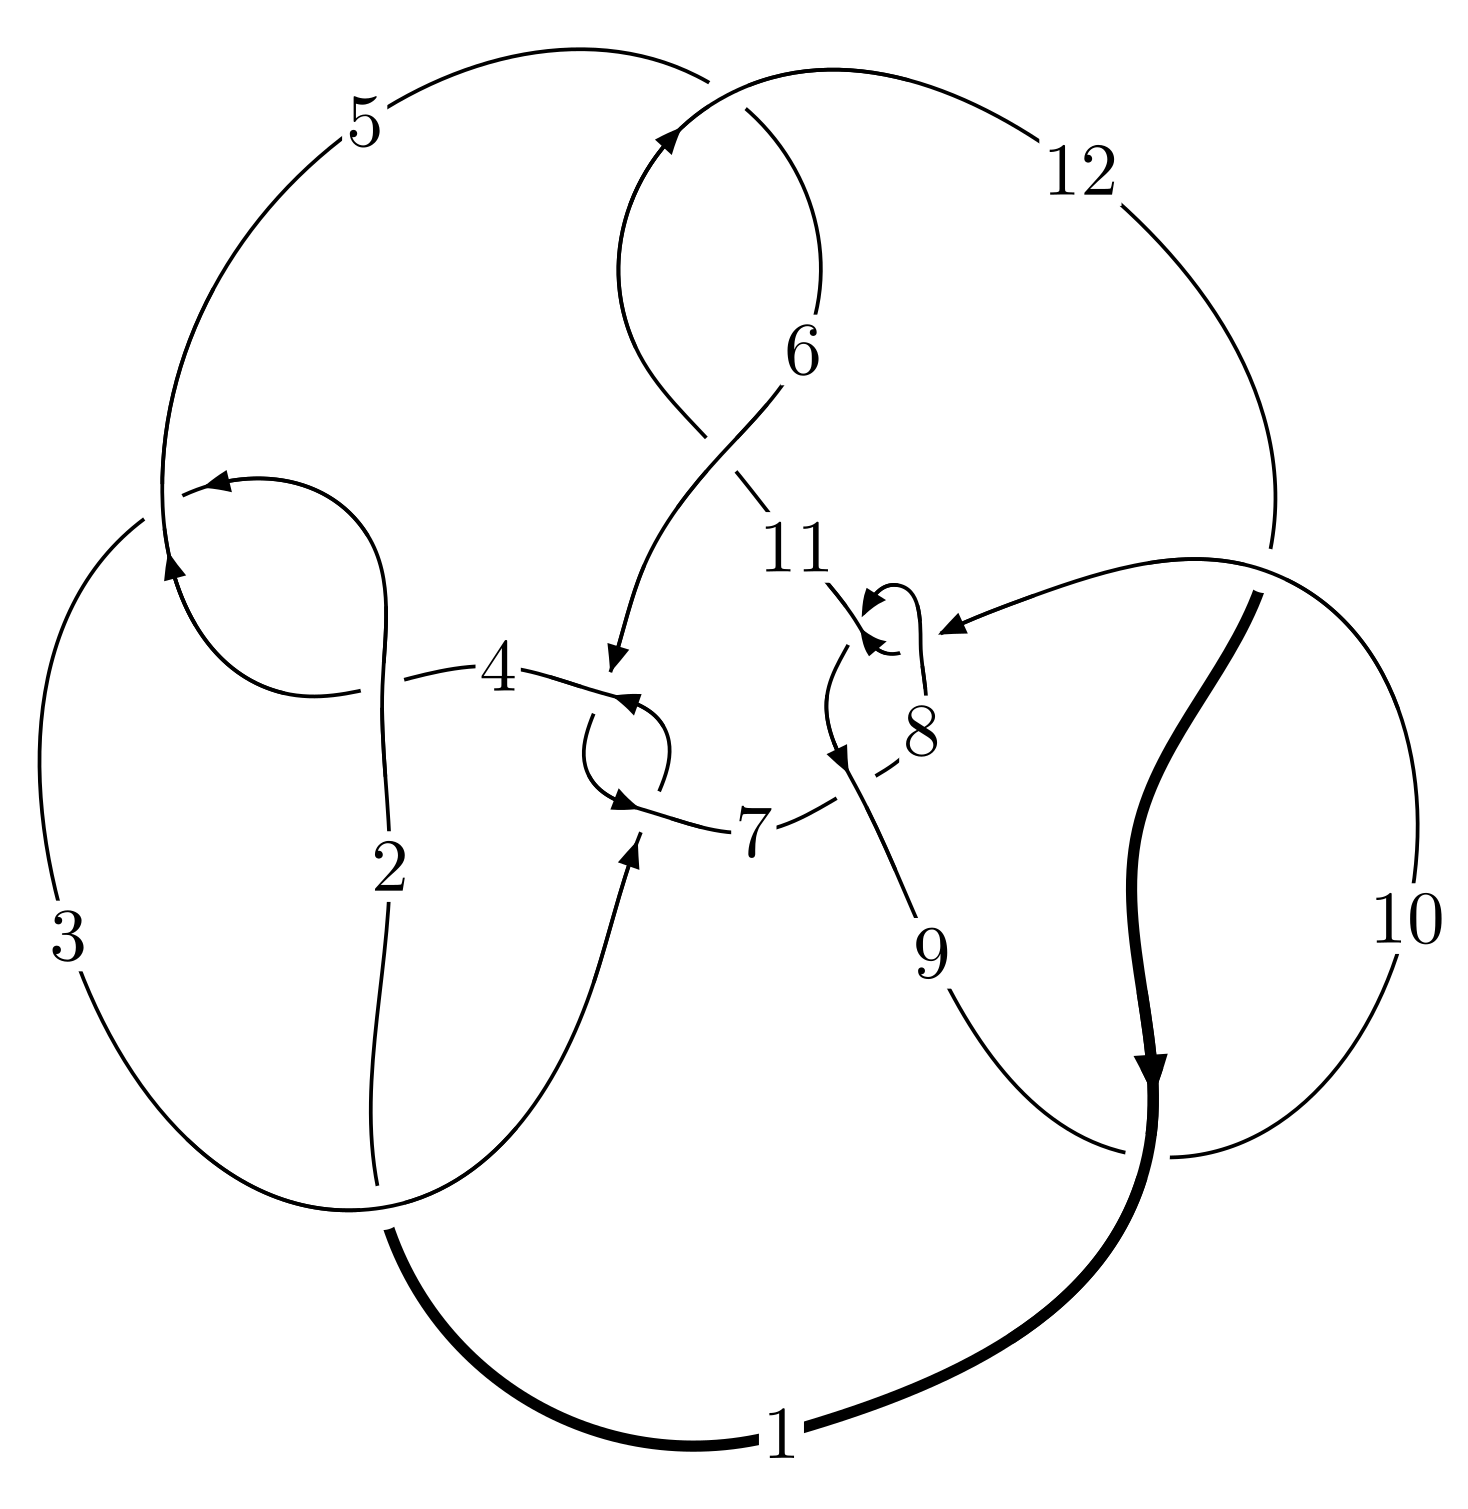
\includegraphics[width=112pt]{../../../GIT/diagram.site/Diagrams/png/865_12a_0064.png}\\
\ \ \ A knot diagram\footnotemark}&
\allowdisplaybreaks
\textbf{Linearized knot diagam} \\
\cline{2-2}
 &
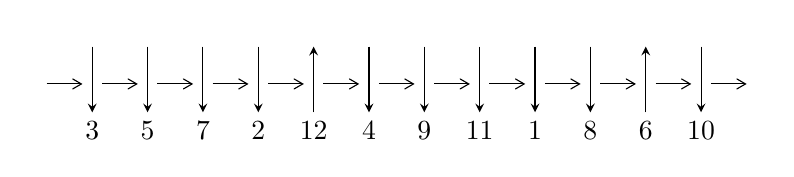
\begin{tikzpicture}[x=20pt, y=17pt]
	% nodes
	\node (C0) at (0, 0) {};
	\node (C1) at (1, 0) {};
	\node (C1U) at (1, +1) {};
	\node (C1D) at (1, -1) {3};

	\node (C2) at (2, 0) {};
	\node (C2U) at (2, +1) {};
	\node (C2D) at (2, -1) {5};

	\node (C3) at (3, 0) {};
	\node (C3U) at (3, +1) {};
	\node (C3D) at (3, -1) {7};

	\node (C4) at (4, 0) {};
	\node (C4U) at (4, +1) {};
	\node (C4D) at (4, -1) {2};

	\node (C5) at (5, 0) {};
	\node (C5U) at (5, +1) {};
	\node (C5D) at (5, -1) {12};

	\node (C6) at (6, 0) {};
	\node (C6U) at (6, +1) {};
	\node (C6D) at (6, -1) {4};

	\node (C7) at (7, 0) {};
	\node (C7U) at (7, +1) {};
	\node (C7D) at (7, -1) {9};

	\node (C8) at (8, 0) {};
	\node (C8U) at (8, +1) {};
	\node (C8D) at (8, -1) {11};

	\node (C9) at (9, 0) {};
	\node (C9U) at (9, +1) {};
	\node (C9D) at (9, -1) {1};

	\node (C10) at (10, 0) {};
	\node (C10U) at (10, +1) {};
	\node (C10D) at (10, -1) {8};

	\node (C11) at (11, 0) {};
	\node (C11U) at (11, +1) {};
	\node (C11D) at (11, -1) {6};

	\node (C12) at (12, 0) {};
	\node (C12U) at (12, +1) {};
	\node (C12D) at (12, -1) {10};
	\node (C13) at (13, 0) {};

	% arrows
	\draw[->,>={angle 60}]
	(C0) edge (C1) (C1) edge (C2) (C2) edge (C3) (C3) edge (C4) (C4) edge (C5) (C5) edge (C6) (C6) edge (C7) (C7) edge (C8) (C8) edge (C9) (C9) edge (C10) (C10) edge (C11) (C11) edge (C12) (C12) edge (C13) ;	\draw[->,>=stealth]
	(C1U) edge (C1D) (C2U) edge (C2D) (C3U) edge (C3D) (C4U) edge (C4D) (C5D) edge (C5U) (C6U) edge (C6D) (C7U) edge (C7D) (C8U) edge (C8D) (C9U) edge (C9D) (C10U) edge (C10D) (C11D) edge (C11U) (C12U) edge (C12D) ;
	\end{tikzpicture} \\
\hhline{~~} \\& 
\textbf{Solving Sequence} \\ \cline{2-2} 
 &
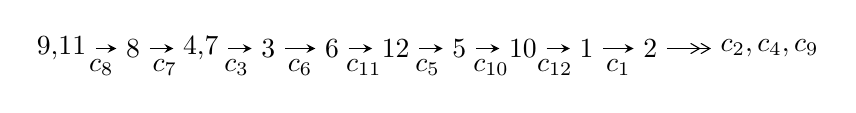
\begin{tikzpicture}[x=23pt, y=7pt]
	% node
	\node (A0) at (-1/8, 0) {9,11};
	\node (A1) at (1, 0) {8};
	\node (A2) at (33/16, 0) {4,7};
	\node (A3) at (25/8, 0) {3};
	\node (A4) at (33/8, 0) {6};
	\node (A5) at (41/8, 0) {12};
	\node (A6) at (49/8, 0) {5};
	\node (A7) at (57/8, 0) {10};
	\node (A8) at (65/8, 0) {1};
	\node (A9) at (73/8, 0) {2};
	\node (C1) at (1/2, -1) {$c_{8}$};
	\node (C2) at (3/2, -1) {$c_{7}$};
	\node (C3) at (21/8, -1) {$c_{3}$};
	\node (C4) at (29/8, -1) {$c_{6}$};
	\node (C5) at (37/8, -1) {$c_{11}$};
	\node (C6) at (45/8, -1) {$c_{5}$};
	\node (C7) at (53/8, -1) {$c_{10}$};
	\node (C8) at (61/8, -1) {$c_{12}$};
	\node (C9) at (69/8, -1) {$c_{1}$};
	\node (A10) at (11, 0) {$c_{2},c_{4},c_{9}$};

	% edge
	\draw[->,>=stealth]	
	(A0) edge (A1) (A1) edge (A2) (A2) edge (A3) (A3) edge (A4) (A4) edge (A5) (A5) edge (A6) (A6) edge (A7) (A7) edge (A8) (A8) edge (A9) ;
	\draw[->>,>={angle 60}]	
	(A9) edge (A10);
\end{tikzpicture} \\ 

\end{tabular} \\

\footnotetext{
The image of knot diagram is generated by the software ``\textbf{Draw programme}" developed by Andrew Bartholomew(\url{http://www.layer8.co.uk/maths/draw/index.htm\#Running-draw}), where we modified some parts for our purpose(\url{https://github.com/CATsTAILs/LinksPainter}).
}\phantom \\ \newline 
\centering \textbf{Ideals for irreducible components\footnotemark of $X_{\text{par}}$} 
 
\begin{align*}
I^u_{1}&=\langle 
-3 u^{19}-8 u^{18}+\cdots+2 b-2,\;u^{20}+2 u^{19}+\cdots+2 a-1,\;u^{21}+3 u^{20}+\cdots-2 u-1\rangle \\
I^u_{2}&=\langle 
-6.83993\times10^{145} u^{113}-6.54937\times10^{146} u^{112}+\cdots+1.45244\times10^{144} b-2.79617\times10^{145},\\
\phantom{I^u_{2}}&\phantom{= \langle  }-7.83619\times10^{145} u^{113}-8.19384\times10^{146} u^{112}+\cdots+2.90489\times10^{144} a-4.22987\times10^{146},\\
\phantom{I^u_{2}}&\phantom{= \langle  }u^{114}+11 u^{113}+\cdots-244 u+1\rangle \\
I^u_{3}&=\langle 
3 u^8+4 u^7-3 u^6-8 u^5-2 u^4+4 u^3+7 u^2+b+5 u+2,\;- u^7-2 u^6+u^5+4 u^4+u^3-3 u^2+a-3 u-2,\\
\phantom{I^u_{3}}&\phantom{= \langle  }u^9+u^8-2 u^7-3 u^6+u^5+3 u^4+2 u^3- u-1\rangle \\
I^u_{4}&=\langle 
-2 a^8+3 a^7-6 a^6+5 a^5-9 a^4+6 a^3-8 a^2+b+3 a-4,\;a^9- a^8+2 a^7- a^6+3 a^5- a^4+2 a^3+a+1,\;u-1\rangle \\
I^u_{5}&=\langle 
u^2+b+u-1,\;a+u,\;u^3+u^2-1\rangle \\
I^u_{6}&=\langle 
4 u^2 a+6 a u+b+4 a+1,\;-2 u^2 a+a^2- a u-2 u^2+2 a- u+2,\;u^3+u^2-1\rangle \\
\\
\end{align*}
\raggedright * 6 irreducible components of $\dim_{\mathbb{C}}=0$, with total 162 representations.\\
\footnotetext{All coefficients of polynomials are rational numbers. But the coefficients are sometimes approximated in decimal forms when there is not enough margin.}
\newpage
\renewcommand{\arraystretch}{1}
\centering \section*{I. $I^u_{1}= \langle -3 u^{19}-8 u^{18}+\cdots+2 b-2,\;u^{20}+2 u^{19}+\cdots+2 a-1,\;u^{21}+3 u^{20}+\cdots-2 u-1 \rangle$}
\flushleft \textbf{(i) Arc colorings}\\
\begin{tabular}{m{7pt} m{180pt} m{7pt} m{180pt} }
\flushright $a_{9}=$&$\begin{pmatrix}1\\0\end{pmatrix}$ \\
\flushright $a_{11}=$&$\begin{pmatrix}0\\u\end{pmatrix}$ \\
\flushright $a_{8}=$&$\begin{pmatrix}1\\- u^2\end{pmatrix}$ \\
\flushright $a_{4}=$&$\begin{pmatrix}-\frac{1}{2} u^{20}- u^{19}+\cdots- u+\frac{1}{2}\\\frac{3}{2} u^{19}+4 u^{18}+\cdots+\frac{5}{2} u+1\end{pmatrix}$ \\
\flushright $a_{7}=$&$\begin{pmatrix}- u^2+1\\- u^2\end{pmatrix}$ \\
\flushright $a_{3}=$&$\begin{pmatrix}-\frac{1}{2} u^{20}-\frac{3}{2} u^{19}+\cdots-\frac{7}{2} u^2-\frac{3}{2} u\\\frac{1}{2} u^{20}+2 u^{19}+\cdots+2 u+\frac{1}{2}\end{pmatrix}$ \\
\flushright $a_{6}=$&$\begin{pmatrix}-\frac{1}{2} u^{20}-\frac{3}{2} u^{19}+\cdots+\frac{1}{2} u+2\\\frac{1}{2} u^{19}+\frac{3}{2} u^{18}+\cdots+\frac{1}{2} u+\frac{1}{2}\end{pmatrix}$ \\
\flushright $a_{12}=$&$\begin{pmatrix}2 u^{20}+4 u^{19}+\cdots-4 u^2-2\\u^{20}+\frac{3}{2} u^{19}+\cdots- u^2+\frac{1}{2} u\end{pmatrix}$ \\
\flushright $a_{5}=$&$\begin{pmatrix}-\frac{5}{2} u^{20}-\frac{11}{2} u^{19}+\cdots+\frac{3}{2} u+3\\\frac{1}{2} u^{18}+u^{17}+\cdots+u+\frac{1}{2}\end{pmatrix}$ \\
\flushright $a_{10}=$&$\begin{pmatrix}u\\- u^3+u\end{pmatrix}$ \\
\flushright $a_{1}=$&$\begin{pmatrix}\frac{5}{2} u^{20}+5 u^{19}+\cdots- u-\frac{5}{2}\\\frac{1}{2} u^{20}+u^{19}+\cdots-3 u^3-\frac{3}{2} u^2\end{pmatrix}$ \\
\flushright $a_{2}=$&$\begin{pmatrix}\frac{5}{2} u^{20}+\frac{11}{2} u^{19}+\cdots-\frac{1}{2} u-\frac{5}{2}\\-\frac{1}{2} u^{20}-\frac{3}{2} u^{19}+\cdots-\frac{3}{2} u-\frac{1}{2}\end{pmatrix}$\\&\end{tabular}
\flushleft \textbf{(ii) Obstruction class $= -1$}\\~\\
\flushleft \textbf{(iii) Cusp Shapes $= -3 u^{20}-19 u^{19}-28 u^{18}+41 u^{17}+153 u^{16}+64 u^{15}-265 u^{14}-364 u^{13}+97 u^{12}+580 u^{11}+342 u^{10}-375 u^9-589 u^8-102 u^7+336 u^6+253 u^5-18 u^4-116 u^3-50 u^2-19 u-11$}\\~\\
\newpage\renewcommand{\arraystretch}{1}
\flushleft \textbf{(iv) u-Polynomials at the component}\newline \\
\begin{tabular}{m{50pt}|m{274pt}}
Crossings & \hspace{64pt}u-Polynomials at each crossing \\
\hline $$\begin{aligned}c_{1},c_{7}\end{aligned}$$&$\begin{aligned}
&u^{21}+11 u^{20}+\cdots-4 u+1
\end{aligned}$\\
\hline $$\begin{aligned}c_{2},c_{4},c_{8}\\c_{10}\end{aligned}$$&$\begin{aligned}
&u^{21}-3 u^{20}+\cdots-2 u+1
\end{aligned}$\\
\hline $$\begin{aligned}c_{3},c_{6},c_{9}\\c_{12}\end{aligned}$$&$\begin{aligned}
&u^{21}- u^{20}+\cdots+4 u+1
\end{aligned}$\\
\hline $$\begin{aligned}c_{5},c_{11}\end{aligned}$$&$\begin{aligned}
&u^{21}+7 u^{20}+\cdots-24 u-8
\end{aligned}$\\
\hline
\end{tabular}\\~\\
\newpage\renewcommand{\arraystretch}{1}
\flushleft \textbf{(v) Riley Polynomials at the component}\newline \\
\begin{tabular}{m{50pt}|m{274pt}}
Crossings & \hspace{64pt}Riley Polynomials at each crossing \\
\hline $$\begin{aligned}c_{1},c_{7}\end{aligned}$$&$\begin{aligned}
&y^{21}+y^{20}+\cdots+60 y-1
\end{aligned}$\\
\hline $$\begin{aligned}c_{2},c_{4},c_{8}\\c_{10}\end{aligned}$$&$\begin{aligned}
&y^{21}-11 y^{20}+\cdots-4 y-1
\end{aligned}$\\
\hline $$\begin{aligned}c_{3},c_{6},c_{9}\\c_{12}\end{aligned}$$&$\begin{aligned}
&y^{21}+9 y^{20}+\cdots+4 y-1
\end{aligned}$\\
\hline $$\begin{aligned}c_{5},c_{11}\end{aligned}$$&$\begin{aligned}
&y^{21}+7 y^{20}+\cdots+384 y-64
\end{aligned}$\\
\hline
\end{tabular}\\~\\
\newpage\flushleft \textbf{(vi) Complex Volumes and Cusp Shapes}
$$\begin{array}{c|c|c}  
\text{Solutions to }I^u_{1}& \I (\text{vol} + \sqrt{-1}CS) & \text{Cusp shape}\\
 \hline 
\begin{aligned}
u &= -0.397532 + 0.952972 I \\
a &= -1.46701 + 1.70855 I \\
b &= -1.64079 + 0.06397 I\end{aligned}
 & \phantom{-}5.42762 - 7.34188 I & -2.93735 + 4.03622 I \\ \hline\begin{aligned}
u &= -0.397532 - 0.952972 I \\
a &= -1.46701 - 1.70855 I \\
b &= -1.64079 - 0.06397 I\end{aligned}
 & \phantom{-}5.42762 + 7.34188 I & -2.93735 - 4.03622 I \\ \hline\begin{aligned}
u &= -0.463906 + 0.848244 I \\
a &= \phantom{-}1.78399 - 0.57848 I \\
b &= \phantom{-}1.53953 + 0.74905 I\end{aligned}
 & \phantom{-}6.79620 - 1.15294 I & -1.115456 - 0.635021 I \\ \hline\begin{aligned}
u &= -0.463906 - 0.848244 I \\
a &= \phantom{-}1.78399 + 0.57848 I \\
b &= \phantom{-}1.53953 - 0.74905 I\end{aligned}
 & \phantom{-}6.79620 + 1.15294 I & -1.115456 + 0.635021 I \\ \hline\begin{aligned}
u &= \phantom{-}0.882297 + 0.334419 I \\
a &= \phantom{-}0.232035 + 1.015740 I \\
b &= \phantom{-}0.473224 - 0.788051 I\end{aligned}
 & -2.27847 - 1.35735 I & -12.26664 + 3.16411 I \\ \hline\begin{aligned}
u &= \phantom{-}0.882297 - 0.334419 I \\
a &= \phantom{-}0.232035 - 1.015740 I \\
b &= \phantom{-}0.473224 + 0.788051 I\end{aligned}
 & -2.27847 + 1.35735 I & -12.26664 - 3.16411 I \\ \hline\begin{aligned}
u &= \phantom{-}0.931344\phantom{ +0.000000I} \\
a &= -1.44830\phantom{ +0.000000I} \\
b &= \phantom{-}6.82396\phantom{ +0.000000I}\end{aligned}
 & -2.88079\phantom{ +0.000000I} & -73.8270\phantom{ +0.000000I} \\ \hline\begin{aligned}
u &= \phantom{-}1.019660 + 0.542496 I \\
a &= \phantom{-}0.251541 + 0.051587 I \\
b &= \phantom{-}0.859784 + 0.625986 I\end{aligned}
 & -4.35380 - 5.94110 I & -11.79339 + 6.03278 I \\ \hline\begin{aligned}
u &= \phantom{-}1.019660 - 0.542496 I \\
a &= \phantom{-}0.251541 - 0.051587 I \\
b &= \phantom{-}0.859784 - 0.625986 I\end{aligned}
 & -4.35380 + 5.94110 I & -11.79339 - 6.03278 I \\ \hline\begin{aligned}
u &= -0.777943 + 0.303148 I \\
a &= -0.536058 + 0.895141 I \\
b &= -0.287676 + 0.330307 I\end{aligned}
 & \phantom{-}0.94396 + 2.98921 I & -0.51194 - 9.40250 I\\
 \hline 
 \end{array}$$\newpage$$\begin{array}{c|c|c}  
\text{Solutions to }I^u_{1}& \I (\text{vol} + \sqrt{-1}CS) & \text{Cusp shape}\\
 \hline 
\begin{aligned}
u &= -0.777943 - 0.303148 I \\
a &= -0.536058 - 0.895141 I \\
b &= -0.287676 - 0.330307 I\end{aligned}
 & \phantom{-}0.94396 - 2.98921 I & -0.51194 + 9.40250 I \\ \hline\begin{aligned}
u &= -1.129490 + 0.380138 I \\
a &= \phantom{-}0.424670 - 0.157361 I \\
b &= -0.322627 - 0.310934 I\end{aligned}
 & -6.57363 + 8.18913 I & -13.0291 - 11.3346 I \\ \hline\begin{aligned}
u &= -1.129490 - 0.380138 I \\
a &= \phantom{-}0.424670 + 0.157361 I \\
b &= -0.322627 + 0.310934 I\end{aligned}
 & -6.57363 - 8.18913 I & -13.0291 + 11.3346 I \\ \hline\begin{aligned}
u &= \phantom{-}1.241170 + 0.210800 I \\
a &= \phantom{-}0.75510 - 1.44309 I \\
b &= \phantom{-}0.44119 - 2.32654 I\end{aligned}
 & -5.92018 + 0.83164 I & -11.63192 - 4.49260 I \\ \hline\begin{aligned}
u &= \phantom{-}1.241170 - 0.210800 I \\
a &= \phantom{-}0.75510 + 1.44309 I \\
b &= \phantom{-}0.44119 + 2.32654 I\end{aligned}
 & -5.92018 - 0.83164 I & -11.63192 + 4.49260 I \\ \hline\begin{aligned}
u &= -1.142470 + 0.607681 I \\
a &= \phantom{-}0.515989 - 1.228650 I \\
b &= \phantom{-}2.19730 - 0.30131 I\end{aligned}
 & \phantom{-}2.55725 + 12.07520 I & -7.44072 - 8.70390 I \\ \hline\begin{aligned}
u &= -1.142470 - 0.607681 I \\
a &= \phantom{-}0.515989 + 1.228650 I \\
b &= \phantom{-}2.19730 + 0.30131 I\end{aligned}
 & \phantom{-}2.55725 - 12.07520 I & -7.44072 + 8.70390 I \\ \hline\begin{aligned}
u &= -1.202640 + 0.655976 I \\
a &= -1.51704 + 0.96579 I \\
b &= -2.94250 - 0.46093 I\end{aligned}
 & \phantom{-}0.4705 + 19.1772 I & -8.57373 - 11.20098 I \\ \hline\begin{aligned}
u &= -1.202640 - 0.655976 I \\
a &= -1.51704 - 0.96579 I \\
b &= -2.94250 + 0.46093 I\end{aligned}
 & \phantom{-}0.4705 - 19.1772 I & -8.57373 + 11.20098 I \\ \hline\begin{aligned}
u &= \phantom{-}0.005183 + 0.428880 I \\
a &= \phantom{-}1.280940 - 0.328547 I \\
b &= -0.229418 - 0.478934 I\end{aligned}
 & -0.56389 - 1.48786 I & -4.78639 + 4.72577 I\\
 \hline 
 \end{array}$$\newpage$$\begin{array}{c|c|c}  
\text{Solutions to }I^u_{1}& \I (\text{vol} + \sqrt{-1}CS) & \text{Cusp shape}\\
 \hline 
\begin{aligned}
u &= \phantom{-}0.005183 - 0.428880 I \\
a &= \phantom{-}1.280940 + 0.328547 I \\
b &= -0.229418 + 0.478934 I\end{aligned}
 & -0.56389 + 1.48786 I & -4.78639 - 4.72577 I\\
 \hline 
 \end{array}$$\newpage\newpage\renewcommand{\arraystretch}{1}
\centering \section*{II. $I^u_{2}= \langle -6.84\times10^{145} u^{113}-6.55\times10^{146} u^{112}+\cdots+1.45\times10^{144} b-2.80\times10^{145},\;-7.84\times10^{145} u^{113}-8.19\times10^{146} u^{112}+\cdots+2.90\times10^{144} a-4.23\times10^{146},\;u^{114}+11 u^{113}+\cdots-244 u+1 \rangle$}
\flushleft \textbf{(i) Arc colorings}\\
\begin{tabular}{m{7pt} m{180pt} m{7pt} m{180pt} }
\flushright $a_{9}=$&$\begin{pmatrix}1\\0\end{pmatrix}$ \\
\flushright $a_{11}=$&$\begin{pmatrix}0\\u\end{pmatrix}$ \\
\flushright $a_{8}=$&$\begin{pmatrix}1\\- u^2\end{pmatrix}$ \\
\flushright $a_{4}=$&$\begin{pmatrix}26.9759 u^{113}+282.071 u^{112}+\cdots-6802.68 u+145.612\\47.0925 u^{113}+450.920 u^{112}+\cdots-4819.75 u+19.2514\end{pmatrix}$ \\
\flushright $a_{7}=$&$\begin{pmatrix}- u^2+1\\- u^2\end{pmatrix}$ \\
\flushright $a_{3}=$&$\begin{pmatrix}-8.42016 u^{113}-58.2813 u^{112}+\cdots-3397.00 u+131.106\\43.1668 u^{113}+438.065 u^{112}+\cdots-9408.31 u+37.9280\end{pmatrix}$ \\
\flushright $a_{6}=$&$\begin{pmatrix}-20.6797 u^{113}-207.500 u^{112}+\cdots+4040.09 u+45.5888\\-4.04307 u^{113}-53.0186 u^{112}+\cdots+2846.86 u-11.8823\end{pmatrix}$ \\
\flushright $a_{12}=$&$\begin{pmatrix}-11.1969 u^{113}-107.084 u^{112}+\cdots+480.862 u+13.6402\\-26.4702 u^{113}-254.764 u^{112}+\cdots+2787.16 u-11.4982\end{pmatrix}$ \\
\flushright $a_{5}=$&$\begin{pmatrix}-46.3066 u^{113}-446.665 u^{112}+\cdots+5731.61 u+42.5602\\-12.0229 u^{113}-108.252 u^{112}+\cdots-163.581 u+0.340418\end{pmatrix}$ \\
\flushright $a_{10}=$&$\begin{pmatrix}u\\- u^3+u\end{pmatrix}$ \\
\flushright $a_{1}=$&$\begin{pmatrix}-5.46063 u^{113}-26.0519 u^{112}+\cdots-4944.78 u+35.7594\\22.1192 u^{113}+237.575 u^{112}+\cdots-7008.51 u+28.5545\end{pmatrix}$ \\
\flushright $a_{2}=$&$\begin{pmatrix}4.26597 u^{113}+40.3853 u^{112}+\cdots-1062.40 u-58.8348\\1.42212 u^{113}+32.2085 u^{112}+\cdots-3675.04 u+15.2628\end{pmatrix}$\\&\end{tabular}
\flushleft \textbf{(ii) Obstruction class $= -1$}\\~\\
\flushleft \textbf{(iii) Cusp Shapes $= 34.1724 u^{113}+358.780 u^{112}+\cdots-9912.17 u+32.0534$}\\~\\
\newpage\renewcommand{\arraystretch}{1}
\flushleft \textbf{(iv) u-Polynomials at the component}\newline \\
\begin{tabular}{m{50pt}|m{274pt}}
Crossings & \hspace{64pt}u-Polynomials at each crossing \\
\hline $$\begin{aligned}c_{1},c_{7}\end{aligned}$$&$\begin{aligned}
&u^{114}+53 u^{113}+\cdots+60814 u+1
\end{aligned}$\\
\hline $$\begin{aligned}c_{2},c_{4},c_{8}\\c_{10}\end{aligned}$$&$\begin{aligned}
&u^{114}-11 u^{113}+\cdots+244 u+1
\end{aligned}$\\
\hline $$\begin{aligned}c_{3},c_{6},c_{9}\\c_{12}\end{aligned}$$&$\begin{aligned}
&u^{114}-4 u^{113}+\cdots+9216 u-512
\end{aligned}$\\
\hline $$\begin{aligned}c_{5},c_{11}\end{aligned}$$&$\begin{aligned}
&(u^{57}-2 u^{56}+\cdots-28 u+8)^{2}
\end{aligned}$\\
\hline
\end{tabular}\\~\\
\newpage\renewcommand{\arraystretch}{1}
\flushleft \textbf{(v) Riley Polynomials at the component}\newline \\
\begin{tabular}{m{50pt}|m{274pt}}
Crossings & \hspace{64pt}Riley Polynomials at each crossing \\
\hline $$\begin{aligned}c_{1},c_{7}\end{aligned}$$&$\begin{aligned}
&y^{114}+27 y^{113}+\cdots-3695912450 y+1
\end{aligned}$\\
\hline $$\begin{aligned}c_{2},c_{4},c_{8}\\c_{10}\end{aligned}$$&$\begin{aligned}
&y^{114}-53 y^{113}+\cdots-60814 y+1
\end{aligned}$\\
\hline $$\begin{aligned}c_{3},c_{6},c_{9}\\c_{12}\end{aligned}$$&$\begin{aligned}
&y^{114}+60 y^{113}+\cdots-63963136 y+262144
\end{aligned}$\\
\hline $$\begin{aligned}c_{5},c_{11}\end{aligned}$$&$\begin{aligned}
&(y^{57}+28 y^{56}+\cdots+976 y-64)^{2}
\end{aligned}$\\
\hline
\end{tabular}\\~\\
\newpage\flushleft \textbf{(vi) Complex Volumes and Cusp Shapes}
$$\begin{array}{c|c|c}  
\text{Solutions to }I^u_{2}& \I (\text{vol} + \sqrt{-1}CS) & \text{Cusp shape}\\
 \hline 
\begin{aligned}
u &= -0.935089 + 0.338704 I \\
a &= \phantom{-}0.850752 + 0.119686 I \\
b &= -0.335249 - 0.500643 I\end{aligned}
 & -5.85242 - 0.17004 I & \phantom{-0.000000 } 0 \\ \hline\begin{aligned}
u &= -0.935089 - 0.338704 I \\
a &= \phantom{-}0.850752 - 0.119686 I \\
b &= -0.335249 + 0.500643 I\end{aligned}
 & -5.85242 + 0.17004 I & \phantom{-0.000000 } 0 \\ \hline\begin{aligned}
u &= -0.363311 + 0.900230 I \\
a &= \phantom{-}0.178573 + 0.463078 I \\
b &= \phantom{-}0.488212 - 0.184046 I\end{aligned}
 & \phantom{-}0.38987 - 6.64143 I & \phantom{-0.000000 } 0 \\ \hline\begin{aligned}
u &= -0.363311 - 0.900230 I \\
a &= \phantom{-}0.178573 - 0.463078 I \\
b &= \phantom{-}0.488212 + 0.184046 I\end{aligned}
 & \phantom{-}0.38987 + 6.64143 I & \phantom{-0.000000 } 0 \\ \hline\begin{aligned}
u &= -0.544457 + 0.799736 I \\
a &= -0.47592 + 1.71750 I \\
b &= -1.232260 - 0.150308 I\end{aligned}
 & \phantom{-}7.34550 - 2.45066 I & \phantom{-0.000000 } 0 \\ \hline\begin{aligned}
u &= -0.544457 - 0.799736 I \\
a &= -0.47592 - 1.71750 I \\
b &= -1.232260 + 0.150308 I\end{aligned}
 & \phantom{-}7.34550 + 2.45066 I & \phantom{-0.000000 } 0 \\ \hline\begin{aligned}
u &= \phantom{-}0.913747 + 0.500557 I \\
a &= -0.446028 - 1.336870 I \\
b &= -2.39965 + 0.30940 I\end{aligned}
 & \phantom{-}2.00680 - 0.99841 I & \phantom{-0.000000 } 0 \\ \hline\begin{aligned}
u &= \phantom{-}0.913747 - 0.500557 I \\
a &= -0.446028 + 1.336870 I \\
b &= -2.39965 - 0.30940 I\end{aligned}
 & \phantom{-}2.00680 + 0.99841 I & \phantom{-0.000000 } 0 \\ \hline\begin{aligned}
u &= -0.974911 + 0.375171 I \\
a &= \phantom{-}1.04389 + 1.21197 I \\
b &= \phantom{-}0.60060 + 1.50246 I\end{aligned}
 & -6.11667 + 2.79727 I & \phantom{-0.000000 } 0 \\ \hline\begin{aligned}
u &= -0.974911 - 0.375171 I \\
a &= \phantom{-}1.04389 - 1.21197 I \\
b &= \phantom{-}0.60060 - 1.50246 I\end{aligned}
 & -6.11667 - 2.79727 I & \phantom{-0.000000 } 0\\
 \hline 
 \end{array}$$\newpage$$\begin{array}{c|c|c}  
\text{Solutions to }I^u_{2}& \I (\text{vol} + \sqrt{-1}CS) & \text{Cusp shape}\\
 \hline 
\begin{aligned}
u &= \phantom{-}0.591439 + 0.742345 I \\
a &= \phantom{-}1.27791 + 1.47235 I \\
b &= \phantom{-}1.96110 - 0.21410 I\end{aligned}
 & -0.66955 + 6.99715 I & \phantom{-0.000000 } 0 \\ \hline\begin{aligned}
u &= \phantom{-}0.591439 - 0.742345 I \\
a &= \phantom{-}1.27791 - 1.47235 I \\
b &= \phantom{-}1.96110 + 0.21410 I\end{aligned}
 & -0.66955 - 6.99715 I & \phantom{-0.000000 } 0 \\ \hline\begin{aligned}
u &= -0.603204 + 0.724752 I \\
a &= \phantom{-}0.08992 - 1.53533 I \\
b &= \phantom{-}1.034000 + 0.309631 I\end{aligned}
 & \phantom{-}6.31677 + 3.78842 I & \phantom{-0.000000 } 0 \\ \hline\begin{aligned}
u &= -0.603204 - 0.724752 I \\
a &= \phantom{-}0.08992 + 1.53533 I \\
b &= \phantom{-}1.034000 - 0.309631 I\end{aligned}
 & \phantom{-}6.31677 - 3.78842 I & \phantom{-0.000000 } 0 \\ \hline\begin{aligned}
u &= -0.361235 + 0.994127 I \\
a &= \phantom{-}1.67677 - 1.55060 I \\
b &= \phantom{-}1.73022 - 0.06071 I\end{aligned}
 & \phantom{-}3.05680 - 13.20750 I & \phantom{-0.000000 } 0 \\ \hline\begin{aligned}
u &= -0.361235 - 0.994127 I \\
a &= \phantom{-}1.67677 + 1.55060 I \\
b &= \phantom{-}1.73022 + 0.06071 I\end{aligned}
 & \phantom{-}3.05680 + 13.20750 I & \phantom{-0.000000 } 0 \\ \hline\begin{aligned}
u &= -0.710294 + 0.785669 I \\
a &= \phantom{-}1.350040 + 0.185786 I \\
b &= \phantom{-}1.107210 + 0.380959 I\end{aligned}
 & \phantom{-}2.57214 + 2.93898 I & \phantom{-0.000000 } 0 \\ \hline\begin{aligned}
u &= -0.710294 - 0.785669 I \\
a &= \phantom{-}1.350040 - 0.185786 I \\
b &= \phantom{-}1.107210 - 0.380959 I\end{aligned}
 & \phantom{-}2.57214 - 2.93898 I & \phantom{-0.000000 } 0 \\ \hline\begin{aligned}
u &= -0.913827 + 0.203758 I \\
a &= \phantom{-}0.77987 + 1.28445 I \\
b &= \phantom{-}0.220732 + 0.951081 I\end{aligned}
 & -5.07109 - 6.54642 I & \phantom{-0.000000 } 0 \\ \hline\begin{aligned}
u &= -0.913827 - 0.203758 I \\
a &= \phantom{-}0.77987 - 1.28445 I \\
b &= \phantom{-}0.220732 - 0.951081 I\end{aligned}
 & -5.07109 + 6.54642 I & \phantom{-0.000000 } 0\\
 \hline 
 \end{array}$$\newpage$$\begin{array}{c|c|c}  
\text{Solutions to }I^u_{2}& \I (\text{vol} + \sqrt{-1}CS) & \text{Cusp shape}\\
 \hline 
\begin{aligned}
u &= \phantom{-}0.934277 + 0.044606 I \\
a &= -1.27302 + 0.62199 I \\
b &= \phantom{-}6.22746 - 0.11628 I\end{aligned}
 & -2.88161\phantom{ +0.000000I} & \phantom{-0.000000 } 0 \\ \hline\begin{aligned}
u &= \phantom{-}0.934277 - 0.044606 I \\
a &= -1.27302 - 0.62199 I \\
b &= \phantom{-}6.22746 + 0.11628 I\end{aligned}
 & -2.88161\phantom{ +0.000000I} & \phantom{-0.000000 } 0 \\ \hline\begin{aligned}
u &= \phantom{-}0.993751 + 0.415165 I \\
a &= -0.202287 - 0.111454 I \\
b &= -0.688804 - 0.887752 I\end{aligned}
 & -2.88934 - 1.48893 I & \phantom{-0.000000 } 0 \\ \hline\begin{aligned}
u &= \phantom{-}0.993751 - 0.415165 I \\
a &= -0.202287 + 0.111454 I \\
b &= -0.688804 + 0.887752 I\end{aligned}
 & -2.88934 + 1.48893 I & \phantom{-0.000000 } 0 \\ \hline\begin{aligned}
u &= -0.607754 + 0.690667 I \\
a &= -2.55750 + 0.99847 I \\
b &= -1.97548 - 1.05995 I\end{aligned}
 & \phantom{-}0.91644 + 1.21025 I & \phantom{-0.000000 } 0 \\ \hline\begin{aligned}
u &= -0.607754 - 0.690667 I \\
a &= -2.55750 - 0.99847 I \\
b &= -1.97548 + 1.05995 I\end{aligned}
 & \phantom{-}0.91644 - 1.21025 I & \phantom{-0.000000 } 0 \\ \hline\begin{aligned}
u &= \phantom{-}0.651838 + 0.645048 I \\
a &= -1.03350 - 1.59021 I \\
b &= -2.00486 + 0.31771 I\end{aligned}
 & \phantom{-}1.42672 + 1.76217 I & \phantom{-0.000000 } 0 \\ \hline\begin{aligned}
u &= \phantom{-}0.651838 - 0.645048 I \\
a &= -1.03350 + 1.59021 I \\
b &= -2.00486 - 0.31771 I\end{aligned}
 & \phantom{-}1.42672 - 1.76217 I & \phantom{-0.000000 } 0 \\ \hline\begin{aligned}
u &= -0.353913 + 0.845498 I \\
a &= \phantom{-}1.40632 - 2.46214 I \\
b &= \phantom{-}1.50509 - 0.30868 I\end{aligned}
 & -0.72077 - 3.96419 I & \phantom{-0.000000 } 0 \\ \hline\begin{aligned}
u &= -0.353913 - 0.845498 I \\
a &= \phantom{-}1.40632 + 2.46214 I \\
b &= \phantom{-}1.50509 + 0.30868 I\end{aligned}
 & -0.72077 + 3.96419 I & \phantom{-0.000000 } 0\\
 \hline 
 \end{array}$$\newpage$$\begin{array}{c|c|c}  
\text{Solutions to }I^u_{2}& \I (\text{vol} + \sqrt{-1}CS) & \text{Cusp shape}\\
 \hline 
\begin{aligned}
u &= -1.003140 + 0.412990 I \\
a &= \phantom{-}0.134567 - 1.062100 I \\
b &= \phantom{-}0.253159 - 0.330157 I\end{aligned}
 & -0.0831767\phantom{ +0.000000I} & \phantom{-0.000000 } 0 \\ \hline\begin{aligned}
u &= -1.003140 - 0.412990 I \\
a &= \phantom{-}0.134567 + 1.062100 I \\
b &= \phantom{-}0.253159 + 0.330157 I\end{aligned}
 & -0.0831767\phantom{ +0.000000I} & \phantom{-0.000000 } 0 \\ \hline\begin{aligned}
u &= -0.882583 + 0.631624 I \\
a &= \phantom{-}0.556823 + 1.098240 I \\
b &= -0.050659 + 0.752253 I\end{aligned}
 & \phantom{-}2.11375 + 2.54354 I & \phantom{-0.000000 } 0 \\ \hline\begin{aligned}
u &= -0.882583 - 0.631624 I \\
a &= \phantom{-}0.556823 - 1.098240 I \\
b &= -0.050659 - 0.752253 I\end{aligned}
 & \phantom{-}2.11375 - 2.54354 I & \phantom{-0.000000 } 0 \\ \hline\begin{aligned}
u &= -0.365682 + 0.836149 I \\
a &= -1.71940 + 0.32564 I \\
b &= -1.43084 - 0.77704 I\end{aligned}
 & \phantom{-}4.87423 - 6.70670 I & \phantom{-0.000000 } 0 \\ \hline\begin{aligned}
u &= -0.365682 - 0.836149 I \\
a &= -1.71940 - 0.32564 I \\
b &= -1.43084 + 0.77704 I\end{aligned}
 & \phantom{-}4.87423 + 6.70670 I & \phantom{-0.000000 } 0 \\ \hline\begin{aligned}
u &= -0.855779 + 0.303645 I \\
a &= -0.788708 - 1.168320 I \\
b &= -0.514747 - 0.982746 I\end{aligned}
 & -1.75595 - 1.61826 I & \phantom{-0.000000 } 0 \\ \hline\begin{aligned}
u &= -0.855779 - 0.303645 I \\
a &= -0.788708 + 1.168320 I \\
b &= -0.514747 + 0.982746 I\end{aligned}
 & -1.75595 + 1.61826 I & \phantom{-0.000000 } 0 \\ \hline\begin{aligned}
u &= -1.001490 + 0.442923 I \\
a &= -0.534520 - 0.168120 I \\
b &= \phantom{-}0.235876 + 0.485155 I\end{aligned}
 & -2.71251 + 4.62043 I & \phantom{-0.000000 } 0 \\ \hline\begin{aligned}
u &= -1.001490 - 0.442923 I \\
a &= -0.534520 + 0.168120 I \\
b &= \phantom{-}0.235876 - 0.485155 I\end{aligned}
 & -2.71251 - 4.62043 I & \phantom{-0.000000 } 0\\
 \hline 
 \end{array}$$\newpage$$\begin{array}{c|c|c}  
\text{Solutions to }I^u_{2}& \I (\text{vol} + \sqrt{-1}CS) & \text{Cusp shape}\\
 \hline 
\begin{aligned}
u &= -0.513607 + 0.741605 I \\
a &= -1.283240 - 0.030725 I \\
b &= -0.982627 + 0.066544 I\end{aligned}
 & \phantom{-}2.00680 - 0.99841 I & \phantom{-0.000000 } 0 \\ \hline\begin{aligned}
u &= -0.513607 - 0.741605 I \\
a &= -1.283240 + 0.030725 I \\
b &= -0.982627 - 0.066544 I\end{aligned}
 & \phantom{-}2.00680 + 0.99841 I & \phantom{-0.000000 } 0 \\ \hline\begin{aligned}
u &= -0.408525 + 0.785138 I \\
a &= -0.141578 - 0.526635 I \\
b &= -0.544167 + 0.043679 I\end{aligned}
 & \phantom{-}1.42672 - 1.76217 I & \phantom{-0.000000 } 0 \\ \hline\begin{aligned}
u &= -0.408525 - 0.785138 I \\
a &= -0.141578 + 0.526635 I \\
b &= -0.544167 - 0.043679 I\end{aligned}
 & \phantom{-}1.42672 + 1.76217 I & \phantom{-0.000000 } 0 \\ \hline\begin{aligned}
u &= -0.092244 + 0.870800 I \\
a &= \phantom{-}0.273591 + 0.305144 I \\
b &= \phantom{-}0.196994 - 0.274279 I\end{aligned}
 & -1.75595 - 1.61826 I & \phantom{-0.000000 } 0 \\ \hline\begin{aligned}
u &= -0.092244 - 0.870800 I \\
a &= \phantom{-}0.273591 - 0.305144 I \\
b &= \phantom{-}0.196994 + 0.274279 I\end{aligned}
 & -1.75595 + 1.61826 I & \phantom{-0.000000 } 0 \\ \hline\begin{aligned}
u &= \phantom{-}1.018750 + 0.476916 I \\
a &= \phantom{-}0.350624 + 1.161860 I \\
b &= \phantom{-}2.48100 - 0.15060 I\end{aligned}
 & \phantom{-}0.39261 - 6.15931 I & \phantom{-0.000000 } 0 \\ \hline\begin{aligned}
u &= \phantom{-}1.018750 - 0.476916 I \\
a &= \phantom{-}0.350624 - 1.161860 I \\
b &= \phantom{-}2.48100 + 0.15060 I\end{aligned}
 & \phantom{-}0.39261 + 6.15931 I & \phantom{-0.000000 } 0 \\ \hline\begin{aligned}
u &= \phantom{-}0.756655 + 0.420921 I \\
a &= \phantom{-}1.214540 + 0.652117 I \\
b &= \phantom{-}1.89236 - 1.84847 I\end{aligned}
 & \phantom{-}2.57214 - 2.93898 I & \phantom{-0.000000 } 0 \\ \hline\begin{aligned}
u &= \phantom{-}0.756655 - 0.420921 I \\
a &= \phantom{-}1.214540 - 0.652117 I \\
b &= \phantom{-}1.89236 + 1.84847 I\end{aligned}
 & \phantom{-}2.57214 + 2.93898 I & \phantom{-0.000000 } 0\\
 \hline 
 \end{array}$$\newpage$$\begin{array}{c|c|c}  
\text{Solutions to }I^u_{2}& \I (\text{vol} + \sqrt{-1}CS) & \text{Cusp shape}\\
 \hline 
\begin{aligned}
u &= -0.685449 + 0.914736 I \\
a &= \phantom{-}1.50544 - 1.21375 I \\
b &= \phantom{-}1.69664 + 0.39127 I\end{aligned}
 & \phantom{-}7.34550 + 2.45066 I & \phantom{-0.000000 } 0 \\ \hline\begin{aligned}
u &= -0.685449 - 0.914736 I \\
a &= \phantom{-}1.50544 + 1.21375 I \\
b &= \phantom{-}1.69664 - 0.39127 I\end{aligned}
 & \phantom{-}7.34550 - 2.45066 I & \phantom{-0.000000 } 0 \\ \hline\begin{aligned}
u &= \phantom{-}1.031590 + 0.492984 I \\
a &= -1.80812 - 0.87554 I \\
b &= -3.16106 + 1.51186 I\end{aligned}
 & -5.22774 - 3.33747 I & \phantom{-0.000000 } 0 \\ \hline\begin{aligned}
u &= \phantom{-}1.031590 - 0.492984 I \\
a &= -1.80812 + 0.87554 I \\
b &= -3.16106 - 1.51186 I\end{aligned}
 & -5.22774 + 3.33747 I & \phantom{-0.000000 } 0 \\ \hline\begin{aligned}
u &= \phantom{-}0.989207 + 0.597613 I \\
a &= \phantom{-}1.46479 + 0.94667 I \\
b &= \phantom{-}2.63360 - 1.11009 I\end{aligned}
 & \phantom{-}0.38987 - 6.64143 I & \phantom{-0.000000 } 0 \\ \hline\begin{aligned}
u &= \phantom{-}0.989207 - 0.597613 I \\
a &= \phantom{-}1.46479 - 0.94667 I \\
b &= \phantom{-}2.63360 + 1.11009 I\end{aligned}
 & \phantom{-}0.38987 + 6.64143 I & \phantom{-0.000000 } 0 \\ \hline\begin{aligned}
u &= \phantom{-}1.138690 + 0.225773 I \\
a &= -0.091897 - 0.232614 I \\
b &= \phantom{-}0.485769 - 1.286550 I\end{aligned}
 & -3.38914 - 0.67754 I & \phantom{-0.000000 } 0 \\ \hline\begin{aligned}
u &= \phantom{-}1.138690 - 0.225773 I \\
a &= -0.091897 + 0.232614 I \\
b &= \phantom{-}0.485769 + 1.286550 I\end{aligned}
 & -3.38914 + 0.67754 I & \phantom{-0.000000 } 0 \\ \hline\begin{aligned}
u &= -1.004000 + 0.595357 I \\
a &= \phantom{-}0.73786 - 1.91783 I \\
b &= \phantom{-}2.55639 - 0.40972 I\end{aligned}
 & -0.28156 + 3.75363 I & \phantom{-0.000000 } 0 \\ \hline\begin{aligned}
u &= -1.004000 - 0.595357 I \\
a &= \phantom{-}0.73786 + 1.91783 I \\
b &= \phantom{-}2.55639 + 0.40972 I\end{aligned}
 & -0.28156 - 3.75363 I & \phantom{-0.000000 } 0\\
 \hline 
 \end{array}$$\newpage$$\begin{array}{c|c|c}  
\text{Solutions to }I^u_{2}& \I (\text{vol} + \sqrt{-1}CS) & \text{Cusp shape}\\
 \hline 
\begin{aligned}
u &= -0.916494 + 0.738189 I \\
a &= \phantom{-}0.26382 + 2.19070 I \\
b &= -0.94011 + 1.28799 I\end{aligned}
 & \phantom{-}1.99622 + 2.68142 I & \phantom{-0.000000 } 0 \\ \hline\begin{aligned}
u &= -0.916494 - 0.738189 I \\
a &= \phantom{-}0.26382 - 2.19070 I \\
b &= -0.94011 - 1.28799 I\end{aligned}
 & \phantom{-}1.99622 - 2.68142 I & \phantom{-0.000000 } 0 \\ \hline\begin{aligned}
u &= -1.002740 + 0.618362 I \\
a &= -1.299220 - 0.163820 I \\
b &= -2.08563 - 1.17049 I\end{aligned}
 & \phantom{-}5.11807 + 1.34577 I & \phantom{-0.000000 } 0 \\ \hline\begin{aligned}
u &= -1.002740 - 0.618362 I \\
a &= -1.299220 + 0.163820 I \\
b &= -2.08563 + 1.17049 I\end{aligned}
 & \phantom{-}5.11807 - 1.34577 I & \phantom{-0.000000 } 0 \\ \hline\begin{aligned}
u &= \phantom{-}0.179685 + 0.801420 I \\
a &= -0.545647 - 0.416620 I \\
b &= -0.086027 + 0.476561 I\end{aligned}
 & -2.71251 - 4.62043 I & \phantom{-0.000000 } 0 \\ \hline\begin{aligned}
u &= \phantom{-}0.179685 - 0.801420 I \\
a &= -0.545647 + 0.416620 I \\
b &= -0.086027 - 0.476561 I\end{aligned}
 & -2.71251 + 4.62043 I & \phantom{-0.000000 } 0 \\ \hline\begin{aligned}
u &= \phantom{-}0.819663\phantom{ +0.000000I} \\
a &= \phantom{-}0.328152\phantom{ +0.000000I} \\
b &= -0.477779\phantom{ +0.000000I}\end{aligned}
 & -1.19406\phantom{ +0.000000I} & \phantom{-0.000000 } 0 \\ \hline\begin{aligned}
u &= -0.760316 + 0.943701 I \\
a &= -1.28155 + 1.33638 I \\
b &= -1.62449 - 0.22495 I\end{aligned}
 & \phantom{-}5.81781 + 7.86530 I & \phantom{-0.000000 } 0 \\ \hline\begin{aligned}
u &= -0.760316 - 0.943701 I \\
a &= -1.28155 - 1.33638 I \\
b &= -1.62449 + 0.22495 I\end{aligned}
 & \phantom{-}5.81781 - 7.86530 I & \phantom{-0.000000 } 0 \\ \hline\begin{aligned}
u &= \phantom{-}1.036360 + 0.631451 I \\
a &= -1.41429 - 1.05458 I \\
b &= -2.66301 + 0.86744 I\end{aligned}
 & -2.02455 - 12.24910 I & \phantom{-0.000000 } 0\\
 \hline 
 \end{array}$$\newpage$$\begin{array}{c|c|c}  
\text{Solutions to }I^u_{2}& \I (\text{vol} + \sqrt{-1}CS) & \text{Cusp shape}\\
 \hline 
\begin{aligned}
u &= \phantom{-}1.036360 - 0.631451 I \\
a &= -1.41429 + 1.05458 I \\
b &= -2.66301 - 0.86744 I\end{aligned}
 & -2.02455 + 12.24910 I & \phantom{-0.000000 } 0 \\ \hline\begin{aligned}
u &= -1.055580 + 0.612560 I \\
a &= \phantom{-}0.024962 - 1.265440 I \\
b &= \phantom{-}0.465183 - 0.429798 I\end{aligned}
 & \phantom{-}0.39261 + 6.15931 I & \phantom{-0.000000 } 0 \\ \hline\begin{aligned}
u &= -1.055580 - 0.612560 I \\
a &= \phantom{-}0.024962 + 1.265440 I \\
b &= \phantom{-}0.465183 + 0.429798 I\end{aligned}
 & \phantom{-}0.39261 - 6.15931 I & \phantom{-0.000000 } 0 \\ \hline\begin{aligned}
u &= \phantom{-}1.210960 + 0.201725 I \\
a &= \phantom{-}0.246902 + 0.934548 I \\
b &= \phantom{-}0.730080 - 0.057414 I\end{aligned}
 & -0.28156 + 3.75363 I & \phantom{-0.000000 } 0 \\ \hline\begin{aligned}
u &= \phantom{-}1.210960 - 0.201725 I \\
a &= \phantom{-}0.246902 - 0.934548 I \\
b &= \phantom{-}0.730080 + 0.057414 I\end{aligned}
 & -0.28156 - 3.75363 I & \phantom{-0.000000 } 0 \\ \hline\begin{aligned}
u &= \phantom{-}1.227000 + 0.083482 I \\
a &= -0.314738 - 0.955394 I \\
b &= -0.929505 - 0.362390 I\end{aligned}
 & \phantom{-}0.91644 - 1.21025 I & \phantom{-0.000000 } 0 \\ \hline\begin{aligned}
u &= \phantom{-}1.227000 - 0.083482 I \\
a &= -0.314738 + 0.955394 I \\
b &= -0.929505 + 0.362390 I\end{aligned}
 & \phantom{-}0.91644 + 1.21025 I & \phantom{-0.000000 } 0 \\ \hline\begin{aligned}
u &= -1.052070 + 0.643114 I \\
a &= \phantom{-}1.43787 - 0.11164 I \\
b &= \phantom{-}2.37341 + 1.12747 I\end{aligned}
 & \phantom{-}5.81781 + 7.86530 I & \phantom{-0.000000 } 0 \\ \hline\begin{aligned}
u &= -1.052070 - 0.643114 I \\
a &= \phantom{-}1.43787 + 0.11164 I \\
b &= \phantom{-}2.37341 - 1.12747 I\end{aligned}
 & \phantom{-}5.81781 - 7.86530 I & \phantom{-0.000000 } 0 \\ \hline\begin{aligned}
u &= \phantom{-}0.517991 + 0.549703 I \\
a &= -0.650153 - 0.900346 I \\
b &= -0.085921 + 0.705389 I\end{aligned}
 & -2.88934 + 1.48893 I & \phantom{-0.000000 } 0\\
 \hline 
 \end{array}$$\newpage$$\begin{array}{c|c|c}  
\text{Solutions to }I^u_{2}& \I (\text{vol} + \sqrt{-1}CS) & \text{Cusp shape}\\
 \hline 
\begin{aligned}
u &= \phantom{-}0.517991 - 0.549703 I \\
a &= -0.650153 + 0.900346 I \\
b &= -0.085921 - 0.705389 I\end{aligned}
 & -2.88934 - 1.48893 I & \phantom{-0.000000 } 0 \\ \hline\begin{aligned}
u &= \phantom{-}0.731384 + 0.164640 I \\
a &= -0.653476 - 0.496177 I \\
b &= -1.48203 + 2.77131 I\end{aligned}
 & \phantom{-}1.99622 + 2.68142 I & \phantom{-0.000000 -}0. + 16.3931 I \\ \hline\begin{aligned}
u &= \phantom{-}0.731384 - 0.164640 I \\
a &= -0.653476 + 0.496177 I \\
b &= -1.48203 - 2.77131 I\end{aligned}
 & \phantom{-}1.99622 - 2.68142 I & \phantom{-0.000000 } 0. - 16.3931 I \\ \hline\begin{aligned}
u &= -1.114310 + 0.603665 I \\
a &= -0.194103 - 0.275883 I \\
b &= -0.173420 + 0.457226 I\end{aligned}
 & -0.66955 + 6.99715 I & \phantom{-0.000000 } 0 \\ \hline\begin{aligned}
u &= -1.114310 - 0.603665 I \\
a &= -0.194103 + 0.275883 I \\
b &= -0.173420 - 0.457226 I\end{aligned}
 & -0.66955 - 6.99715 I & \phantom{-0.000000 } 0 \\ \hline\begin{aligned}
u &= -1.104900 + 0.647613 I \\
a &= -0.72162 + 1.28759 I \\
b &= -2.27486 + 0.23636 I\end{aligned}
 & \phantom{-}4.87423 + 6.70670 I & \phantom{-0.000000 } 0 \\ \hline\begin{aligned}
u &= -1.104900 - 0.647613 I \\
a &= -0.72162 - 1.28759 I \\
b &= -2.27486 - 0.23636 I\end{aligned}
 & \phantom{-}4.87423 - 6.70670 I & \phantom{-0.000000 } 0 \\ \hline\begin{aligned}
u &= \phantom{-}1.201390 + 0.483404 I \\
a &= \phantom{-}0.164242 - 0.057254 I \\
b &= \phantom{-}0.711703 + 0.194974 I\end{aligned}
 & -5.85242 - 0.17004 I & \phantom{-0.000000 } 0 \\ \hline\begin{aligned}
u &= \phantom{-}1.201390 - 0.483404 I \\
a &= \phantom{-}0.164242 + 0.057254 I \\
b &= \phantom{-}0.711703 - 0.194974 I\end{aligned}
 & -5.85242 + 0.17004 I & \phantom{-0.000000 } 0 \\ \hline\begin{aligned}
u &= -1.028230 + 0.790978 I \\
a &= -1.31506 + 0.93346 I \\
b &= -2.23776 - 0.11435 I\end{aligned}
 & \phantom{-}6.31677 + 3.78842 I & \phantom{-0.000000 } 0\\
 \hline 
 \end{array}$$\newpage$$\begin{array}{c|c|c}  
\text{Solutions to }I^u_{2}& \I (\text{vol} + \sqrt{-1}CS) & \text{Cusp shape}\\
 \hline 
\begin{aligned}
u &= -1.028230 - 0.790978 I \\
a &= -1.31506 - 0.93346 I \\
b &= -2.23776 + 0.11435 I\end{aligned}
 & \phantom{-}6.31677 - 3.78842 I & \phantom{-0.000000 } 0 \\ \hline\begin{aligned}
u &= \phantom{-}1.285900 + 0.178551 I \\
a &= -0.021664 + 0.315043 I \\
b &= -1.18986 + 0.88462 I\end{aligned}
 & -5.22774 + 3.33747 I & \phantom{-0.000000 } 0 \\ \hline\begin{aligned}
u &= \phantom{-}1.285900 - 0.178551 I \\
a &= -0.021664 - 0.315043 I \\
b &= -1.18986 - 0.88462 I\end{aligned}
 & -5.22774 - 3.33747 I & \phantom{-0.000000 } 0 \\ \hline\begin{aligned}
u &= -1.147930 + 0.609222 I \\
a &= -1.97009 + 0.65340 I \\
b &= -3.16991 - 1.05389 I\end{aligned}
 & -3.08563 + 9.35831 I & \phantom{-0.000000 } 0 \\ \hline\begin{aligned}
u &= -1.147930 - 0.609222 I \\
a &= -1.97009 - 0.65340 I \\
b &= -3.16991 + 1.05389 I\end{aligned}
 & -3.08563 - 9.35831 I & \phantom{-0.000000 } 0 \\ \hline\begin{aligned}
u &= -0.993984 + 0.853696 I \\
a &= \phantom{-}1.40031 - 0.65532 I \\
b &= \phantom{-}2.08860 + 0.21266 I\end{aligned}
 & \phantom{-}5.11807 - 1.34577 I & \phantom{-0.000000 } 0 \\ \hline\begin{aligned}
u &= -0.993984 - 0.853696 I \\
a &= \phantom{-}1.40031 + 0.65532 I \\
b &= \phantom{-}2.08860 - 0.21266 I\end{aligned}
 & \phantom{-}5.11807 + 1.34577 I & \phantom{-0.000000 } 0 \\ \hline\begin{aligned}
u &= -1.207130 + 0.510791 I \\
a &= -0.024746 + 0.196336 I \\
b &= \phantom{-}0.239684 - 0.075811 I\end{aligned}
 & -5.07109 + 6.54642 I & \phantom{-0.000000 } 0 \\ \hline\begin{aligned}
u &= -1.207130 - 0.510791 I \\
a &= -0.024746 - 0.196336 I \\
b &= \phantom{-}0.239684 + 0.075811 I\end{aligned}
 & -5.07109 - 6.54642 I & \phantom{-0.000000 } 0 \\ \hline\begin{aligned}
u &= -1.163600 + 0.628049 I \\
a &= \phantom{-}0.142909 + 0.301527 I \\
b &= \phantom{-}0.289119 - 0.406103 I\end{aligned}
 & -2.02455 + 12.24910 I & \phantom{-0.000000 } 0\\
 \hline 
 \end{array}$$\newpage$$\begin{array}{c|c|c}  
\text{Solutions to }I^u_{2}& \I (\text{vol} + \sqrt{-1}CS) & \text{Cusp shape}\\
 \hline 
\begin{aligned}
u &= -1.163600 - 0.628049 I \\
a &= \phantom{-}0.142909 - 0.301527 I \\
b &= \phantom{-}0.289119 + 0.406103 I\end{aligned}
 & -2.02455 - 12.24910 I & \phantom{-0.000000 } 0 \\ \hline\begin{aligned}
u &= \phantom{-}1.332370 + 0.130005 I \\
a &= -0.391141 + 1.285310 I \\
b &= -0.209248 + 1.386280 I\end{aligned}
 & -0.72077 + 3.96419 I & \phantom{-0.000000 } 0 \\ \hline\begin{aligned}
u &= \phantom{-}1.332370 - 0.130005 I \\
a &= -0.391141 - 1.285310 I \\
b &= -0.209248 - 1.386280 I\end{aligned}
 & -0.72077 - 3.96419 I & \phantom{-0.000000 } 0 \\ \hline\begin{aligned}
u &= \phantom{-}1.288330 + 0.366402 I \\
a &= -0.096677 + 0.174502 I \\
b &= -0.820998 + 0.303703 I\end{aligned}
 & -6.11667 - 2.79727 I & \phantom{-0.000000 } 0 \\ \hline\begin{aligned}
u &= \phantom{-}1.288330 - 0.366402 I \\
a &= -0.096677 - 0.174502 I \\
b &= -0.820998 - 0.303703 I\end{aligned}
 & -6.11667 + 2.79727 I & \phantom{-0.000000 } 0 \\ \hline\begin{aligned}
u &= -1.173290 + 0.657195 I \\
a &= \phantom{-}1.57584 - 0.80785 I \\
b &= \phantom{-}2.90418 + 0.65113 I\end{aligned}
 & \phantom{-}3.05680 + 13.20750 I & \phantom{-0.000000 } 0 \\ \hline\begin{aligned}
u &= -1.173290 - 0.657195 I \\
a &= \phantom{-}1.57584 + 0.80785 I \\
b &= \phantom{-}2.90418 - 0.65113 I\end{aligned}
 & \phantom{-}3.05680 - 13.20750 I & \phantom{-0.000000 } 0 \\ \hline\begin{aligned}
u &= \phantom{-}1.377950 + 0.169180 I \\
a &= \phantom{-}0.294813 - 1.373240 I \\
b &= -0.140571 - 1.374840 I\end{aligned}
 & -3.08563 + 9.35831 I & \phantom{-0.000000 } 0 \\ \hline\begin{aligned}
u &= \phantom{-}1.377950 - 0.169180 I \\
a &= \phantom{-}0.294813 + 1.373240 I \\
b &= -0.140571 + 1.374840 I\end{aligned}
 & -3.08563 - 9.35831 I & \phantom{-0.000000 } 0 \\ \hline\begin{aligned}
u &= \phantom{-}0.337881 + 0.475409 I \\
a &= \phantom{-}1.49606 + 2.67220 I \\
b &= \phantom{-}1.46334 - 0.31833 I\end{aligned}
 & -3.38914 - 0.67754 I & -11.03837 - 0.57218 I\\
 \hline 
 \end{array}$$\newpage$$\begin{array}{c|c|c}  
\text{Solutions to }I^u_{2}& \I (\text{vol} + \sqrt{-1}CS) & \text{Cusp shape}\\
 \hline 
\begin{aligned}
u &= \phantom{-}0.337881 - 0.475409 I \\
a &= \phantom{-}1.49606 - 2.67220 I \\
b &= \phantom{-}1.46334 + 0.31833 I\end{aligned}
 & -3.38914 + 0.67754 I & -11.03837 + 0.57218 I \\ \hline\begin{aligned}
u &= \phantom{-}0.242095 + 0.261744 I \\
a &= -1.75583 - 1.65677 I \\
b &= -0.638812 + 1.260710 I\end{aligned}
 & \phantom{-}2.11375 + 2.54354 I & -0.09108 - 1.48335 I \\ \hline\begin{aligned}
u &= \phantom{-}0.242095 - 0.261744 I \\
a &= -1.75583 + 1.65677 I \\
b &= -0.638812 - 1.260710 I\end{aligned}
 & \phantom{-}2.11375 - 2.54354 I & -0.09108 + 1.48335 I \\ \hline\begin{aligned}
u &= \phantom{-}0.00405574\phantom{ +0.000000I} \\
a &= \phantom{-}117.803\phantom{ +0.000000I} \\
b &= -0.520574\phantom{ +0.000000I}\end{aligned}
 & -1.19406\phantom{ +0.000000I} & -8.42600\phantom{ +0.000000I}\\
 \hline 
 \end{array}$$\newpage\newpage\renewcommand{\arraystretch}{1}
\centering \section*{III. $I^u_{3}= \langle 3 u^8+4 u^7+\cdots+b+2,\;- u^7-2 u^6+u^5+4 u^4+u^3-3 u^2+a-3 u-2,\;u^9+u^8-2 u^7-3 u^6+u^5+3 u^4+2 u^3- u-1 \rangle$}
\flushleft \textbf{(i) Arc colorings}\\
\begin{tabular}{m{7pt} m{180pt} m{7pt} m{180pt} }
\flushright $a_{9}=$&$\begin{pmatrix}1\\0\end{pmatrix}$ \\
\flushright $a_{11}=$&$\begin{pmatrix}0\\u\end{pmatrix}$ \\
\flushright $a_{8}=$&$\begin{pmatrix}1\\- u^2\end{pmatrix}$ \\
\flushright $a_{4}=$&$\begin{pmatrix}u^7+2 u^6- u^5-4 u^4- u^3+3 u^2+3 u+2\\-3 u^8-4 u^7+3 u^6+8 u^5+2 u^4-4 u^3-7 u^2-5 u-2\end{pmatrix}$ \\
\flushright $a_{7}=$&$\begin{pmatrix}- u^2+1\\- u^2\end{pmatrix}$ \\
\flushright $a_{3}=$&$\begin{pmatrix}u^7+2 u^6- u^5-4 u^4- u^3+3 u^2+3 u+2\\-3 u^8-4 u^7+3 u^6+8 u^5+2 u^4-4 u^3-7 u^2-5 u-2\end{pmatrix}$ \\
\flushright $a_{6}=$&$\begin{pmatrix}- u^2+1\\- u^2\end{pmatrix}$ \\
\flushright $a_{12}=$&$\begin{pmatrix}u^5-2 u^3+u\\u^5- u^3+u\end{pmatrix}$ \\
\flushright $a_{5}=$&$\begin{pmatrix}- u^8+3 u^6-3 u^4+1\\- u^8+2 u^6-2 u^4\end{pmatrix}$ \\
\flushright $a_{10}=$&$\begin{pmatrix}u\\- u^3+u\end{pmatrix}$ \\
\flushright $a_{1}=$&$\begin{pmatrix}u^8-3 u^6+3 u^4-1\\u^8-2 u^6+2 u^4\end{pmatrix}$ \\
\flushright $a_{2}=$&$\begin{pmatrix}u^8+u^7- u^6- u^5- u^4- u^3+3 u^2+3 u+1\\-2 u^8-4 u^7+u^6+8 u^5+4 u^4-4 u^3-7 u^2-5 u-2\end{pmatrix}$\\&\end{tabular}
\flushleft \textbf{(ii) Obstruction class $= 1$}\\~\\
\flushleft \textbf{(iii) Cusp Shapes $= 42 u^8+74 u^7-19 u^6-137 u^5-75 u^4+54 u^3+135 u^2+112 u+44$}\\~\\
\newpage\renewcommand{\arraystretch}{1}
\flushleft \textbf{(iv) u-Polynomials at the component}\newline \\
\begin{tabular}{m{50pt}|m{274pt}}
Crossings & \hspace{64pt}u-Polynomials at each crossing \\
\hline $$\begin{aligned}c_{1},c_{2}\end{aligned}$$&$\begin{aligned}
&(u-1)^9
\end{aligned}$\\
\hline $$\begin{aligned}c_{3},c_{6}\end{aligned}$$&$\begin{aligned}
&u^9
\end{aligned}$\\
\hline $$\begin{aligned}c_{4}\end{aligned}$$&$\begin{aligned}
&(u+1)^9
\end{aligned}$\\
\hline $$\begin{aligned}c_{5}\end{aligned}$$&$\begin{aligned}
&u^9+3 u^8+8 u^7+13 u^6+17 u^5+17 u^4+12 u^3+6 u^2+u-1
\end{aligned}$\\
\hline $$\begin{aligned}c_{7}\end{aligned}$$&$\begin{aligned}
&u^9-5 u^8+12 u^7-15 u^6+9 u^5+u^4-4 u^3+2 u^2+u-1
\end{aligned}$\\
\hline $$\begin{aligned}c_{8}\end{aligned}$$&$\begin{aligned}
&u^9+u^8-2 u^7-3 u^6+u^5+3 u^4+2 u^3- u-1
\end{aligned}$\\
\hline $$\begin{aligned}c_{9}\end{aligned}$$&$\begin{aligned}
&u^9+u^8+2 u^7+u^6+3 u^5+u^4+2 u^3+u-1
\end{aligned}$\\
\hline $$\begin{aligned}c_{10}\end{aligned}$$&$\begin{aligned}
&u^9- u^8-2 u^7+3 u^6+u^5-3 u^4+2 u^3- u+1
\end{aligned}$\\
\hline $$\begin{aligned}c_{11}\end{aligned}$$&$\begin{aligned}
&u^9-3 u^8+8 u^7-13 u^6+17 u^5-17 u^4+12 u^3-6 u^2+u+1
\end{aligned}$\\
\hline $$\begin{aligned}c_{12}\end{aligned}$$&$\begin{aligned}
&u^9- u^8+2 u^7- u^6+3 u^5- u^4+2 u^3+u+1
\end{aligned}$\\
\hline
\end{tabular}\\~\\
\newpage\renewcommand{\arraystretch}{1}
\flushleft \textbf{(v) Riley Polynomials at the component}\newline \\
\begin{tabular}{m{50pt}|m{274pt}}
Crossings & \hspace{64pt}Riley Polynomials at each crossing \\
\hline $$\begin{aligned}c_{1},c_{2},c_{4}\end{aligned}$$&$\begin{aligned}
&(y-1)^9
\end{aligned}$\\
\hline $$\begin{aligned}c_{3},c_{6}\end{aligned}$$&$\begin{aligned}
&y^9
\end{aligned}$\\
\hline $$\begin{aligned}c_{5},c_{11}\end{aligned}$$&$\begin{aligned}
&y^9+7 y^8+20 y^7+25 y^6+5 y^5-15 y^4+22 y^2+13 y-1
\end{aligned}$\\
\hline $$\begin{aligned}c_{7}\end{aligned}$$&$\begin{aligned}
&y^9- y^8+12 y^7-7 y^6+37 y^5+y^4-10 y^2+5 y-1
\end{aligned}$\\
\hline $$\begin{aligned}c_{8},c_{10}\end{aligned}$$&$\begin{aligned}
&y^9-5 y^8+12 y^7-15 y^6+9 y^5+y^4-4 y^3+2 y^2+y-1
\end{aligned}$\\
\hline $$\begin{aligned}c_{9},c_{12}\end{aligned}$$&$\begin{aligned}
&y^9+3 y^8+8 y^7+13 y^6+17 y^5+17 y^4+12 y^3+6 y^2+y-1
\end{aligned}$\\
\hline
\end{tabular}\\~\\
\newpage\flushleft \textbf{(vi) Complex Volumes and Cusp Shapes}
$$\begin{array}{c|c|c}  
\text{Solutions to }I^u_{3}& \I (\text{vol} + \sqrt{-1}CS) & \text{Cusp shape}\\
 \hline 
\begin{aligned}
u &= -0.772920 + 0.510351 I \\
a &= \phantom{-}1.082180 + 0.329167 I \\
b &= \phantom{-}0.162031 + 0.927542 I\end{aligned}
 & \phantom{-}0.13850 + 2.09337 I & -6.65973 - 4.50528 I \\ \hline\begin{aligned}
u &= -0.772920 - 0.510351 I \\
a &= \phantom{-}1.082180 - 0.329167 I \\
b &= \phantom{-}0.162031 - 0.927542 I\end{aligned}
 & \phantom{-}0.13850 - 2.09337 I & -6.65973 + 4.50528 I \\ \hline\begin{aligned}
u &= \phantom{-}0.825933\phantom{ +0.000000I} \\
a &= \phantom{-}4.61221\phantom{ +0.000000I} \\
b &= -9.89910\phantom{ +0.000000I}\end{aligned}
 & -2.84338\phantom{ +0.000000I} & \phantom{-}193.930\phantom{ +0.000000I} \\ \hline\begin{aligned}
u &= \phantom{-}1.173910 + 0.391555 I \\
a &= \phantom{-}0.271310 + 0.634428 I \\
b &= \phantom{-}0.990590 + 0.515152 I\end{aligned}
 & -6.01628 - 1.33617 I & -13.00050 + 1.13735 I \\ \hline\begin{aligned}
u &= \phantom{-}1.173910 - 0.391555 I \\
a &= \phantom{-}0.271310 - 0.634428 I \\
b &= \phantom{-}0.990590 - 0.515152 I\end{aligned}
 & -6.01628 + 1.33617 I & -13.00050 - 1.13735 I \\ \hline\begin{aligned}
u &= -0.141484 + 0.739668 I \\
a &= -0.996034 + 0.562654 I \\
b &= -0.405386 + 0.113252 I\end{aligned}
 & -2.26187 - 2.45442 I & -9.69685 + 4.13179 I \\ \hline\begin{aligned}
u &= -0.141484 - 0.739668 I \\
a &= -0.996034 - 0.562654 I \\
b &= -0.405386 - 0.113252 I\end{aligned}
 & -2.26187 + 2.45442 I & -9.69685 - 4.13179 I \\ \hline\begin{aligned}
u &= -1.172470 + 0.500383 I \\
a &= \phantom{-}0.336447 - 0.398473 I \\
b &= \phantom{-}0.702315 - 0.150499 I\end{aligned}
 & -5.24306 + 7.08493 I & -11.6081 - 10.4867 I \\ \hline\begin{aligned}
u &= -1.172470 - 0.500383 I \\
a &= \phantom{-}0.336447 + 0.398473 I \\
b &= \phantom{-}0.702315 + 0.150499 I\end{aligned}
 & -5.24306 - 7.08493 I & -11.6081 + 10.4867 I\\
 \hline 
 \end{array}$$\newpage\newpage\renewcommand{\arraystretch}{1}
\centering \section*{IV. $I^u_{4}= \langle -2 a^8+b+\cdots+3 a-4,\;a^9- a^8+2 a^7- a^6+3 a^5- a^4+2 a^3+a+1,\;u-1 \rangle$}
\flushleft \textbf{(i) Arc colorings}\\
\begin{tabular}{m{7pt} m{180pt} m{7pt} m{180pt} }
\flushright $a_{9}=$&$\begin{pmatrix}1\\0\end{pmatrix}$ \\
\flushright $a_{11}=$&$\begin{pmatrix}0\\1\end{pmatrix}$ \\
\flushright $a_{8}=$&$\begin{pmatrix}1\\-1\end{pmatrix}$ \\
\flushright $a_{4}=$&$\begin{pmatrix}a\\2 a^8-3 a^7+6 a^6-5 a^5+9 a^4-6 a^3+8 a^2-3 a+4\end{pmatrix}$ \\
\flushright $a_{7}=$&$\begin{pmatrix}0\\-1\end{pmatrix}$ \\
\flushright $a_{3}=$&$\begin{pmatrix}a\\2 a^8-3 a^7+6 a^6-5 a^5+9 a^4-6 a^3+8 a^2-4 a+4\end{pmatrix}$ \\
\flushright $a_{6}=$&$\begin{pmatrix}- a^2\\a^8-2 a^7+3 a^6-3 a^5+4 a^4-4 a^3+3 a^2-2 a+1\end{pmatrix}$ \\
\flushright $a_{12}=$&$\begin{pmatrix}a^4\\0\end{pmatrix}$ \\
\flushright $a_{5}=$&$\begin{pmatrix}- a^6- a^2\\a^8-2 a^7+3 a^6-3 a^5+4 a^4-4 a^3+3 a^2-2 a+1\end{pmatrix}$ \\
\flushright $a_{10}=$&$\begin{pmatrix}1\\0\end{pmatrix}$ \\
\flushright $a_{1}=$&$\begin{pmatrix}a^4\\0\end{pmatrix}$ \\
\flushright $a_{2}=$&$\begin{pmatrix}- a^6- a^2\\a^8-2 a^7+4 a^6-3 a^5+6 a^4-4 a^3+6 a^2-2 a+3\end{pmatrix}$\\&\end{tabular}
\flushleft \textbf{(ii) Obstruction class $= 1$}\\~\\
\flushleft \textbf{(iii) Cusp Shapes $= 45 a^8-63 a^7+119 a^6-104 a^5+184 a^4-133 a^3+157 a^2-83 a+73$}\\~\\
\newpage\renewcommand{\arraystretch}{1}
\flushleft \textbf{(iv) u-Polynomials at the component}\newline \\
\begin{tabular}{m{50pt}|m{274pt}}
Crossings & \hspace{64pt}u-Polynomials at each crossing \\
\hline $$\begin{aligned}c_{1}\end{aligned}$$&$\begin{aligned}
&u^9-5 u^8+12 u^7-15 u^6+9 u^5+u^4-4 u^3+2 u^2+u-1
\end{aligned}$\\
\hline $$\begin{aligned}c_{2}\end{aligned}$$&$\begin{aligned}
&u^9+u^8-2 u^7-3 u^6+u^5+3 u^4+2 u^3- u-1
\end{aligned}$\\
\hline $$\begin{aligned}c_{3}\end{aligned}$$&$\begin{aligned}
&u^9+u^8+2 u^7+u^6+3 u^5+u^4+2 u^3+u-1
\end{aligned}$\\
\hline $$\begin{aligned}c_{4}\end{aligned}$$&$\begin{aligned}
&u^9- u^8-2 u^7+3 u^6+u^5-3 u^4+2 u^3- u+1
\end{aligned}$\\
\hline $$\begin{aligned}c_{5}\end{aligned}$$&$\begin{aligned}
&u^9-3 u^8+8 u^7-13 u^6+17 u^5-17 u^4+12 u^3-6 u^2+u+1
\end{aligned}$\\
\hline $$\begin{aligned}c_{6}\end{aligned}$$&$\begin{aligned}
&u^9- u^8+2 u^7- u^6+3 u^5- u^4+2 u^3+u+1
\end{aligned}$\\
\hline $$\begin{aligned}c_{7},c_{8}\end{aligned}$$&$\begin{aligned}
&(u-1)^9
\end{aligned}$\\
\hline $$\begin{aligned}c_{9},c_{12}\end{aligned}$$&$\begin{aligned}
&u^9
\end{aligned}$\\
\hline $$\begin{aligned}c_{10}\end{aligned}$$&$\begin{aligned}
&(u+1)^9
\end{aligned}$\\
\hline $$\begin{aligned}c_{11}\end{aligned}$$&$\begin{aligned}
&u^9+3 u^8+8 u^7+13 u^6+17 u^5+17 u^4+12 u^3+6 u^2+u-1
\end{aligned}$\\
\hline
\end{tabular}\\~\\
\newpage\renewcommand{\arraystretch}{1}
\flushleft \textbf{(v) Riley Polynomials at the component}\newline \\
\begin{tabular}{m{50pt}|m{274pt}}
Crossings & \hspace{64pt}Riley Polynomials at each crossing \\
\hline $$\begin{aligned}c_{1}\end{aligned}$$&$\begin{aligned}
&y^9- y^8+12 y^7-7 y^6+37 y^5+y^4-10 y^2+5 y-1
\end{aligned}$\\
\hline $$\begin{aligned}c_{2},c_{4}\end{aligned}$$&$\begin{aligned}
&y^9-5 y^8+12 y^7-15 y^6+9 y^5+y^4-4 y^3+2 y^2+y-1
\end{aligned}$\\
\hline $$\begin{aligned}c_{3},c_{6}\end{aligned}$$&$\begin{aligned}
&y^9+3 y^8+8 y^7+13 y^6+17 y^5+17 y^4+12 y^3+6 y^2+y-1
\end{aligned}$\\
\hline $$\begin{aligned}c_{5},c_{11}\end{aligned}$$&$\begin{aligned}
&y^9+7 y^8+20 y^7+25 y^6+5 y^5-15 y^4+22 y^2+13 y-1
\end{aligned}$\\
\hline $$\begin{aligned}c_{7},c_{8},c_{10}\end{aligned}$$&$\begin{aligned}
&(y-1)^9
\end{aligned}$\\
\hline $$\begin{aligned}c_{9},c_{12}\end{aligned}$$&$\begin{aligned}
&y^9
\end{aligned}$\\
\hline
\end{tabular}\\~\\
\newpage\flushleft \textbf{(vi) Complex Volumes and Cusp Shapes}
$$\begin{array}{c|c|c}  
\text{Solutions to }I^u_{4}& \I (\text{vol} + \sqrt{-1}CS) & \text{Cusp shape}\\
 \hline 
\begin{aligned}
u &= \phantom{-}1.00000\phantom{ +0.000000I} \\
a &= -0.140343 + 0.966856 I \\
b &= -0.302374 + 0.039314 I\end{aligned}
 & \phantom{-}0.13850 + 2.09337 I & -6.65973 - 4.50528 I \\ \hline\begin{aligned}
u &= \phantom{-}1.00000\phantom{ +0.000000I} \\
a &= -0.140343 - 0.966856 I \\
b &= -0.302374 - 0.039314 I\end{aligned}
 & \phantom{-}0.13850 - 2.09337 I & -6.65973 + 4.50528 I \\ \hline\begin{aligned}
u &= \phantom{-}1.00000\phantom{ +0.000000I} \\
a &= -0.628449 + 0.875112 I \\
b &= -0.223063 + 0.988364 I\end{aligned}
 & -2.26187 + 2.45442 I & -9.69685 - 4.13179 I \\ \hline\begin{aligned}
u &= \phantom{-}1.00000\phantom{ +0.000000I} \\
a &= -0.628449 - 0.875112 I \\
b &= -0.223063 - 0.988364 I\end{aligned}
 & -2.26187 - 2.45442 I & -9.69685 + 4.13179 I \\ \hline\begin{aligned}
u &= \phantom{-}1.00000\phantom{ +0.000000I} \\
a &= \phantom{-}0.796005 + 0.733148 I \\
b &= -0.194585 + 1.248300 I\end{aligned}
 & -6.01628 + 1.33617 I & -13.00050 - 1.13735 I \\ \hline\begin{aligned}
u &= \phantom{-}1.00000\phantom{ +0.000000I} \\
a &= \phantom{-}0.796005 - 0.733148 I \\
b &= -0.194585 - 1.248300 I\end{aligned}
 & -6.01628 - 1.33617 I & -13.00050 + 1.13735 I \\ \hline\begin{aligned}
u &= \phantom{-}1.00000\phantom{ +0.000000I} \\
a &= \phantom{-}0.728966 + 0.986295 I \\
b &= \phantom{-}0.026651 + 0.835796 I\end{aligned}
 & -5.24306 - 7.08493 I & -11.6081 + 10.4867 I \\ \hline\begin{aligned}
u &= \phantom{-}1.00000\phantom{ +0.000000I} \\
a &= \phantom{-}0.728966 - 0.986295 I \\
b &= \phantom{-}0.026651 - 0.835796 I\end{aligned}
 & -5.24306 + 7.08493 I & -11.6081 - 10.4867 I \\ \hline\begin{aligned}
u &= \phantom{-}1.00000\phantom{ +0.000000I} \\
a &= -0.512358\phantom{ +0.000000I} \\
b &= \phantom{-}9.38674\phantom{ +0.000000I}\end{aligned}
 & -2.84338\phantom{ +0.000000I} & \phantom{-}193.930\phantom{ +0.000000I}\\
 \hline 
 \end{array}$$\newpage\newpage\renewcommand{\arraystretch}{1}
\centering \section*{V. $I^u_{5}= \langle u^2+b+u-1,\;a+u,\;u^3+u^2-1 \rangle$}
\flushleft \textbf{(i) Arc colorings}\\
\begin{tabular}{m{7pt} m{180pt} m{7pt} m{180pt} }
\flushright $a_{9}=$&$\begin{pmatrix}1\\0\end{pmatrix}$ \\
\flushright $a_{11}=$&$\begin{pmatrix}0\\u\end{pmatrix}$ \\
\flushright $a_{8}=$&$\begin{pmatrix}1\\- u^2\end{pmatrix}$ \\
\flushright $a_{4}=$&$\begin{pmatrix}- u\\- u^2- u+1\end{pmatrix}$ \\
\flushright $a_{7}=$&$\begin{pmatrix}- u^2+1\\- u^2\end{pmatrix}$ \\
\flushright $a_{3}=$&$\begin{pmatrix}-1\\0\end{pmatrix}$ \\
\flushright $a_{6}=$&$\begin{pmatrix}0\\- u\end{pmatrix}$ \\
\flushright $a_{12}=$&$\begin{pmatrix}0\\u\end{pmatrix}$ \\
\flushright $a_{5}=$&$\begin{pmatrix}0\\- u\end{pmatrix}$ \\
\flushright $a_{10}=$&$\begin{pmatrix}u\\u^2+u-1\end{pmatrix}$ \\
\flushright $a_{1}=$&$\begin{pmatrix}u^2-1\\u^2\end{pmatrix}$ \\
\flushright $a_{2}=$&$\begin{pmatrix}-1\\u^2\end{pmatrix}$\\&\end{tabular}
\flushleft \textbf{(ii) Obstruction class $= 1$}\\~\\
\flushleft \textbf{(iii) Cusp Shapes $= -8 u-12$}\\~\\
\newpage\renewcommand{\arraystretch}{1}
\flushleft \textbf{(iv) u-Polynomials at the component}\newline \\
\begin{tabular}{m{50pt}|m{274pt}}
Crossings & \hspace{64pt}u-Polynomials at each crossing \\
\hline $$\begin{aligned}c_{1},c_{3},c_{7}\\c_{9}\end{aligned}$$&$\begin{aligned}
&u^3- u^2+2 u-1
\end{aligned}$\\
\hline $$\begin{aligned}c_{2},c_{8}\end{aligned}$$&$\begin{aligned}
&u^3+u^2-1
\end{aligned}$\\
\hline $$\begin{aligned}c_{4},c_{10}\end{aligned}$$&$\begin{aligned}
&u^3- u^2+1
\end{aligned}$\\
\hline $$\begin{aligned}c_{5},c_{11}\end{aligned}$$&$\begin{aligned}
&u^3
\end{aligned}$\\
\hline $$\begin{aligned}c_{6},c_{12}\end{aligned}$$&$\begin{aligned}
&u^3+u^2+2 u+1
\end{aligned}$\\
\hline
\end{tabular}\\~\\
\newpage\renewcommand{\arraystretch}{1}
\flushleft \textbf{(v) Riley Polynomials at the component}\newline \\
\begin{tabular}{m{50pt}|m{274pt}}
Crossings & \hspace{64pt}Riley Polynomials at each crossing \\
\hline $$\begin{aligned}c_{1},c_{3},c_{6}\\c_{7},c_{9},c_{12}\end{aligned}$$&$\begin{aligned}
&y^3+3 y^2+2 y-1
\end{aligned}$\\
\hline $$\begin{aligned}c_{2},c_{4},c_{8}\\c_{10}\end{aligned}$$&$\begin{aligned}
&y^3- y^2+2 y-1
\end{aligned}$\\
\hline $$\begin{aligned}c_{5},c_{11}\end{aligned}$$&$\begin{aligned}
&y^3
\end{aligned}$\\
\hline
\end{tabular}\\~\\
\newpage\flushleft \textbf{(vi) Complex Volumes and Cusp Shapes}
$$\begin{array}{c|c|c}  
\text{Solutions to }I^u_{5}& \I (\text{vol} + \sqrt{-1}CS) & \text{Cusp shape}\\
 \hline 
\begin{aligned}
u &= -0.877439 + 0.744862 I \\
a &= \phantom{-}0.877439 - 0.744862 I \\
b &= \phantom{-}1.66236 + 0.56228 I\end{aligned}
 & \phantom{-}6.04826 + 5.65624 I & -4.98049 - 5.95889 I \\ \hline\begin{aligned}
u &= -0.877439 - 0.744862 I \\
a &= \phantom{-}0.877439 + 0.744862 I \\
b &= \phantom{-}1.66236 - 0.56228 I\end{aligned}
 & \phantom{-}6.04826 - 5.65624 I & -4.98049 + 5.95889 I \\ \hline\begin{aligned}
u &= \phantom{-}0.754878\phantom{ +0.000000I} \\
a &= -0.754878\phantom{ +0.000000I} \\
b &= -0.324718\phantom{ +0.000000I}\end{aligned}
 & -2.22691\phantom{ +0.000000I} & -18.0390\phantom{ +0.000000I}\\
 \hline 
 \end{array}$$\newpage\newpage\renewcommand{\arraystretch}{1}
\centering \section*{VI. $I^u_{6}= \langle 4 u^2 a+6 a u+b+4 a+1,\;-2 u^2 a+a^2- a u-2 u^2+2 a- u+2,\;u^3+u^2-1 \rangle$}
\flushleft \textbf{(i) Arc colorings}\\
\begin{tabular}{m{7pt} m{180pt} m{7pt} m{180pt} }
\flushright $a_{9}=$&$\begin{pmatrix}1\\0\end{pmatrix}$ \\
\flushright $a_{11}=$&$\begin{pmatrix}0\\u\end{pmatrix}$ \\
\flushright $a_{8}=$&$\begin{pmatrix}1\\- u^2\end{pmatrix}$ \\
\flushright $a_{4}=$&$\begin{pmatrix}a\\-4 u^2 a-6 a u-4 a-1\end{pmatrix}$ \\
\flushright $a_{7}=$&$\begin{pmatrix}- u^2+1\\- u^2\end{pmatrix}$ \\
\flushright $a_{3}=$&$\begin{pmatrix}- a u+u^2- u\\-3 u^2 a-5 a u-3 a- u\end{pmatrix}$ \\
\flushright $a_{6}=$&$\begin{pmatrix}0\\- u^2 a-2 a u+2 u^2-2 a+2 u+1\end{pmatrix}$ \\
\flushright $a_{12}=$&$\begin{pmatrix}0\\u\end{pmatrix}$ \\
\flushright $a_{5}=$&$\begin{pmatrix}0\\- u^2 a-2 a u+2 u^2-2 a+2 u+1\end{pmatrix}$ \\
\flushright $a_{10}=$&$\begin{pmatrix}u\\u^2+u-1\end{pmatrix}$ \\
\flushright $a_{1}=$&$\begin{pmatrix}u^2-1\\u^2\end{pmatrix}$ \\
\flushright $a_{2}=$&$\begin{pmatrix}- a u+u^2- u\\- u^2 a-2 a u+2 u^2- a+u+2\end{pmatrix}$\\&\end{tabular}
\flushleft \textbf{(ii) Obstruction class $= 1$}\\~\\
\flushleft \textbf{(iii) Cusp Shapes $= 24 u^2 a+29 a u+29 a-19 u-15$}\\~\\
\newpage\renewcommand{\arraystretch}{1}
\flushleft \textbf{(iv) u-Polynomials at the component}\newline \\
\begin{tabular}{m{50pt}|m{274pt}}
Crossings & \hspace{64pt}u-Polynomials at each crossing \\
\hline $$\begin{aligned}c_{1},c_{3},c_{7}\\c_{9}\end{aligned}$$&$\begin{aligned}
&(u^3- u^2+2 u-1)^2
\end{aligned}$\\
\hline $$\begin{aligned}c_{2},c_{8}\end{aligned}$$&$\begin{aligned}
&(u^3+u^2-1)^2
\end{aligned}$\\
\hline $$\begin{aligned}c_{4},c_{10}\end{aligned}$$&$\begin{aligned}
&(u^3- u^2+1)^2
\end{aligned}$\\
\hline $$\begin{aligned}c_{5},c_{11}\end{aligned}$$&$\begin{aligned}
&u^6
\end{aligned}$\\
\hline $$\begin{aligned}c_{6},c_{12}\end{aligned}$$&$\begin{aligned}
&(u^3+u^2+2 u+1)^2
\end{aligned}$\\
\hline
\end{tabular}\\~\\
\newpage\renewcommand{\arraystretch}{1}
\flushleft \textbf{(v) Riley Polynomials at the component}\newline \\
\begin{tabular}{m{50pt}|m{274pt}}
Crossings & \hspace{64pt}Riley Polynomials at each crossing \\
\hline $$\begin{aligned}c_{1},c_{3},c_{6}\\c_{7},c_{9},c_{12}\end{aligned}$$&$\begin{aligned}
&(y^3+3 y^2+2 y-1)^2
\end{aligned}$\\
\hline $$\begin{aligned}c_{2},c_{4},c_{8}\\c_{10}\end{aligned}$$&$\begin{aligned}
&(y^3- y^2+2 y-1)^2
\end{aligned}$\\
\hline $$\begin{aligned}c_{5},c_{11}\end{aligned}$$&$\begin{aligned}
&y^6
\end{aligned}$\\
\hline
\end{tabular}\\~\\
\newpage\flushleft \textbf{(vi) Complex Volumes and Cusp Shapes}
$$\begin{array}{c|c|c}  
\text{Solutions to }I^u_{6}& \I (\text{vol} + \sqrt{-1}CS) & \text{Cusp shape}\\
 \hline 
\begin{aligned}
u &= -0.877439 + 0.744862 I \\
a &= -1.069840 + 0.424452 I \\
b &= -1.75488 - 0.64082 I\end{aligned}
 & \phantom{-}6.04826\phantom{ +0.000000I} & -3.50653 + 0. I\phantom{ +0.000000I} \\ \hline\begin{aligned}
u &= -0.877439 + 0.744862 I \\
a &= -1.37744 - 2.29387 I \\
b &= \phantom{-}0.18504 - 1.97346 I\end{aligned}
 & \phantom{-}1.91067 + 2.82812 I & -32.7467 - 20.6881 I \\ \hline\begin{aligned}
u &= -0.877439 - 0.744862 I \\
a &= -1.069840 - 0.424452 I \\
b &= -1.75488 + 0.64082 I\end{aligned}
 & \phantom{-}6.04826\phantom{ +0.000000I} & -3.50653 + 0. I\phantom{ +0.000000I} \\ \hline\begin{aligned}
u &= -0.877439 - 0.744862 I \\
a &= -1.37744 + 2.29387 I \\
b &= \phantom{-}0.18504 + 1.97346 I\end{aligned}
 & \phantom{-}1.91067 - 2.82812 I & -32.7467 + 20.6881 I \\ \hline\begin{aligned}
u &= \phantom{-}0.754878\phantom{ +0.000000I} \\
a &= -0.052721 + 0.320410 I \\
b &= -0.43016 - 3.46319 I\end{aligned}
 & \phantom{-}1.91067 - 2.82812 I & -32.7467 + 20.6881 I \\ \hline\begin{aligned}
u &= \phantom{-}0.754878\phantom{ +0.000000I} \\
a &= -0.052721 - 0.320410 I \\
b &= -0.43016 + 3.46319 I\end{aligned}
 & \phantom{-}1.91067 + 2.82812 I & -32.7467 - 20.6881 I\\
 \hline 
 \end{array}$$\newpage
\newpage\renewcommand{\arraystretch}{1}
\centering \section*{ VII. u-Polynomials}
\begin{tabular}{m{50pt}|m{274pt}}
Crossings & \hspace{64pt}u-Polynomials at each crossing \\
\hline $$\begin{aligned}c_{1},c_{7}\end{aligned}$$&$\begin{aligned}
&(u-1)^9(u^3- u^2+2 u-1)^3\\
&\cdot(u^9-5 u^8+12 u^7-15 u^6+9 u^5+u^4-4 u^3+2 u^2+u-1)\\
&\cdot(u^{21}+11 u^{20}+\cdots-4 u+1)(u^{114}+53 u^{113}+\cdots+60814 u+1)
\end{aligned}$\\
\hline $$\begin{aligned}c_{2},c_{8}\end{aligned}$$&$\begin{aligned}
&(u-1)^9(u^3+u^2-1)^3(u^9+u^8-2 u^7-3 u^6+u^5+3 u^4+2 u^3- u-1)\\
&\cdot(u^{21}-3 u^{20}+\cdots-2 u+1)(u^{114}-11 u^{113}+\cdots+244 u+1)
\end{aligned}$\\
\hline $$\begin{aligned}c_{3},c_{9}\end{aligned}$$&$\begin{aligned}
&u^9(u^3- u^2+2 u-1)^3(u^9+u^8+2 u^7+u^6+3 u^5+u^4+2 u^3+u-1)\\
&\cdot(u^{21}- u^{20}+\cdots+4 u+1)(u^{114}-4 u^{113}+\cdots+9216 u-512)
\end{aligned}$\\
\hline $$\begin{aligned}c_{4},c_{10}\end{aligned}$$&$\begin{aligned}
&(u+1)^9(u^3- u^2+1)^3(u^9- u^8-2 u^7+3 u^6+u^5-3 u^4+2 u^3- u+1)\\
&\cdot(u^{21}-3 u^{20}+\cdots-2 u+1)(u^{114}-11 u^{113}+\cdots+244 u+1)
\end{aligned}$\\
\hline $$\begin{aligned}c_{5},c_{11}\end{aligned}$$&$\begin{aligned}
&u^9(u^9-3 u^8+8 u^7-13 u^6+17 u^5-17 u^4+12 u^3-6 u^2+u+1)\\
&\cdot(u^9+3 u^8+8 u^7+13 u^6+17 u^5+17 u^4+12 u^3+6 u^2+u-1)\\
&\cdot(u^{21}+7 u^{20}+\cdots-24 u-8)(u^{57}-2 u^{56}+\cdots-28 u+8)^{2}
\end{aligned}$\\
\hline $$\begin{aligned}c_{6},c_{12}\end{aligned}$$&$\begin{aligned}
&u^9(u^3+u^2+2 u+1)^3(u^9- u^8+2 u^7- u^6+3 u^5- u^4+2 u^3+u+1)\\
&\cdot(u^{21}- u^{20}+\cdots+4 u+1)(u^{114}-4 u^{113}+\cdots+9216 u-512)
\end{aligned}$\\
\hline
\end{tabular}\newpage\renewcommand{\arraystretch}{1}
\centering \section*{ VIII. Riley Polynomials}
\begin{tabular}{m{50pt}|m{274pt}}
Crossings & \hspace{64pt}Riley Polynomials at each crossing \\
\hline $$\begin{aligned}c_{1},c_{7}\end{aligned}$$&$\begin{aligned}
&(y-1)^9(y^3+3 y^2+2 y-1)^3\\
&\cdot(y^9- y^8+12 y^7-7 y^6+37 y^5+y^4-10 y^2+5 y-1)\\
&\cdot(y^{21}+y^{20}+\cdots+60 y-1)(y^{114}+27 y^{113}+\cdots-3695912450 y+1)
\end{aligned}$\\
\hline $$\begin{aligned}c_{2},c_{4},c_{8}\\c_{10}\end{aligned}$$&$\begin{aligned}
&(y-1)^9(y^3- y^2+2 y-1)^3\\
&\cdot(y^9-5 y^8+12 y^7-15 y^6+9 y^5+y^4-4 y^3+2 y^2+y-1)\\
&\cdot(y^{21}-11 y^{20}+\cdots-4 y-1)(y^{114}-53 y^{113}+\cdots-60814 y+1)
\end{aligned}$\\
\hline $$\begin{aligned}c_{3},c_{6},c_{9}\\c_{12}\end{aligned}$$&$\begin{aligned}
&y^9(y^3+3 y^2+2 y-1)^3\\
&\cdot(y^9+3 y^8+8 y^7+13 y^6+17 y^5+17 y^4+12 y^3+6 y^2+y-1)\\
&\cdot(y^{21}+9 y^{20}+\cdots+4 y-1)\\
&\cdot(y^{114}+60 y^{113}+\cdots-63963136 y+262144)
\end{aligned}$\\
\hline $$\begin{aligned}c_{5},c_{11}\end{aligned}$$&$\begin{aligned}
&y^9(y^9+7 y^8+20 y^7+25 y^6+5 y^5-15 y^4+22 y^2+13 y-1)^2\\
&\cdot(y^{21}+7 y^{20}+\cdots+384 y-64)(y^{57}+28 y^{56}+\cdots+976 y-64)^{2}
\end{aligned}$\\
\hline
\end{tabular}
\vskip 2pc
\end{document}